\documentclass{book}
\usepackage[a4paper,top=2.5cm,bottom=2.5cm,left=2.5cm,right=2.5cm]{geometry}
\usepackage{makeidx}
\usepackage{natbib}
\usepackage{graphicx}
\usepackage{multicol}
\usepackage{float}
\usepackage{listings}
\usepackage{color}
\usepackage{ifthen}
\usepackage[table]{xcolor}
\usepackage{textcomp}
\usepackage{alltt}
\usepackage{ifpdf}
\ifpdf
\usepackage[pdftex,
            pagebackref=true,
            colorlinks=true,
            linkcolor=blue,
            unicode
           ]{hyperref}
\else
\usepackage[ps2pdf,
            pagebackref=true,
            colorlinks=true,
            linkcolor=blue,
            unicode
           ]{hyperref}
\usepackage{pspicture}
\fi
\usepackage[utf8]{inputenc}
\usepackage{mathptmx}
\usepackage[scaled=.90]{helvet}
\usepackage{courier}
\usepackage{sectsty}
\usepackage[titles]{tocloft}
\usepackage{doxygen}
\lstset{language=C++,inputencoding=utf8,basicstyle=\footnotesize,breaklines=true,breakatwhitespace=true,tabsize=4,numbers=left }
\makeindex
\setcounter{tocdepth}{3}
\renewcommand{\footrulewidth}{0.4pt}
\renewcommand{\familydefault}{\sfdefault}
\hfuzz=15pt
\setlength{\emergencystretch}{15pt}
\hbadness=750
\tolerance=750
\begin{document}
\hypersetup{pageanchor=false,citecolor=blue}
\begin{titlepage}
\vspace*{7cm}
\begin{center}
{\Large Home\-Coming }\\
\vspace*{1cm}
{\large 作成: Doxygen 1.8.0}\\
\vspace*{0.5cm}
{\small Thu May 24 2012 06:31:20}\\
\end{center}
\end{titlepage}
\clearemptydoublepage
\pagenumbering{roman}
\tableofcontents
\clearemptydoublepage
\pagenumbering{arabic}
\hypersetup{pageanchor=true,citecolor=blue}
\chapter{構成索引}
\section{クラス階層}
この継承一覧はおおまかにはソートされていますが、完全にアルファベット順でソートされてはいません。\begin{DoxyCompactList}
\item \contentsline{section}{Action}{\pageref{class_action}}{}
\item \contentsline{section}{Action\-Table\-Data}{\pageref{interface_action_table_data}}{}
\item \contentsline{section}{App\-Delegate}{\pageref{interface_app_delegate}}{}
\item \contentsline{section}{Command\-Menu\-Controller}{\pageref{interface_command_menu_controller}}{}
\item \contentsline{section}{Game}{\pageref{class_game}}{}
\item \contentsline{section}{Game\-State\-Age}{\pageref{class_game_state_age}}{}
\begin{DoxyCompactList}
\item \contentsline{section}{Lower\-Grades\-Of\-Elementary}{\pageref{class_lower_grades_of_elementary}}{}
\item \contentsline{section}{Upper\-Grades\-Of\-Elementary}{\pageref{class_upper_grades_of_elementary}}{}
\end{DoxyCompactList}
\item \contentsline{section}{Hero}{\pageref{class_hero}}{}
\item \contentsline{section}{Heroine}{\pageref{class_heroine}}{}
\item \contentsline{section}{Heroine\-Attr}{\pageref{class_heroine_attr}}{}
\item \contentsline{section}{Heroine\-Table\-Data}{\pageref{interface_heroine_table_data}}{}
\item \contentsline{section}{Range\-Number}{\pageref{struct_range_number}}{}
\item \contentsline{section}{School}{\pageref{class_school}}{}
\item \contentsline{section}{Story}{\pageref{class_story}}{}
\item \contentsline{section}{Story\-View}{\pageref{interface_story_view}}{}
\item \contentsline{section}{Story\-Window\-Controller}{\pageref{interface_story_window_controller}}{}
\item \contentsline{section}{System}{\pageref{class_system}}{}
\end{DoxyCompactList}

\chapter{構成索引}
\section{構成}
クラス、構造体、共用体、インタフェースの説明です。\begin{DoxyCompactList}
\item\contentsline{section}{\hyperlink{class_action}{Action} }{\pageref{class_action}}{}
\item\contentsline{section}{\hyperlink{interface_action_table_data}{Action\-Table\-Data} }{\pageref{interface_action_table_data}}{}
\item\contentsline{section}{\hyperlink{interface_app_delegate}{App\-Delegate} }{\pageref{interface_app_delegate}}{}
\item\contentsline{section}{\hyperlink{interface_command_menu_controller}{Command\-Menu\-Controller} }{\pageref{interface_command_menu_controller}}{}
\item\contentsline{section}{\hyperlink{class_game}{Game} }{\pageref{class_game}}{}
\item\contentsline{section}{\hyperlink{class_game_state_age}{Game\-State\-Age} }{\pageref{class_game_state_age}}{}
\item\contentsline{section}{\hyperlink{class_hero}{Hero} }{\pageref{class_hero}}{}
\item\contentsline{section}{\hyperlink{class_heroine}{Heroine} }{\pageref{class_heroine}}{}
\item\contentsline{section}{\hyperlink{class_heroine_attr}{Heroine\-Attr} }{\pageref{class_heroine_attr}}{}
\item\contentsline{section}{\hyperlink{interface_heroine_table_data}{Heroine\-Table\-Data} }{\pageref{interface_heroine_table_data}}{}
\item\contentsline{section}{\hyperlink{class_lower_grades_of_elementary}{Lower\-Grades\-Of\-Elementary} }{\pageref{class_lower_grades_of_elementary}}{}
\item\contentsline{section}{\hyperlink{struct_range_number}{Range\-Number} }{\pageref{struct_range_number}}{}
\item\contentsline{section}{\hyperlink{class_school}{School} }{\pageref{class_school}}{}
\item\contentsline{section}{\hyperlink{class_story}{Story} }{\pageref{class_story}}{}
\item\contentsline{section}{\hyperlink{interface_story_view}{Story\-View} }{\pageref{interface_story_view}}{}
\item\contentsline{section}{\hyperlink{interface_story_window_controller}{Story\-Window\-Controller} }{\pageref{interface_story_window_controller}}{}
\item\contentsline{section}{\hyperlink{class_system}{System} }{\pageref{class_system}}{}
\item\contentsline{section}{\hyperlink{class_upper_grades_of_elementary}{Upper\-Grades\-Of\-Elementary} }{\pageref{class_upper_grades_of_elementary}}{}
\end{DoxyCompactList}

\chapter{ファイル索引}
\section{ファイル一覧}
これはファイル一覧です。\begin{DoxyCompactList}
\item\contentsline{section}{Home\-Coming/\hyperlink{_action_8cpp}{Action.\-cpp} }{\pageref{_action_8cpp}}{}
\item\contentsline{section}{Home\-Coming/\hyperlink{_action_8h}{Action.\-h} }{\pageref{_action_8h}}{}
\item\contentsline{section}{Home\-Coming/\hyperlink{_action_table_data_8h}{Action\-Table\-Data.\-h} }{\pageref{_action_table_data_8h}}{}
\item\contentsline{section}{Home\-Coming/\hyperlink{_action_table_data_8mm}{Action\-Table\-Data.\-mm} }{\pageref{_action_table_data_8mm}}{}
\item\contentsline{section}{Home\-Coming/\hyperlink{_app_delegate_8h}{App\-Delegate.\-h} }{\pageref{_app_delegate_8h}}{}
\item\contentsline{section}{Home\-Coming/\hyperlink{_app_delegate_8mm}{App\-Delegate.\-mm} }{\pageref{_app_delegate_8mm}}{}
\item\contentsline{section}{Home\-Coming/\hyperlink{_command_menu_controller_8h}{Command\-Menu\-Controller.\-h} }{\pageref{_command_menu_controller_8h}}{}
\item\contentsline{section}{Home\-Coming/\hyperlink{_command_menu_controller_8mm}{Command\-Menu\-Controller.\-mm} }{\pageref{_command_menu_controller_8mm}}{}
\item\contentsline{section}{Home\-Coming/\hyperlink{_game_8cpp}{Game.\-cpp} }{\pageref{_game_8cpp}}{}
\item\contentsline{section}{Home\-Coming/\hyperlink{_game_8h}{Game.\-h} }{\pageref{_game_8h}}{}
\item\contentsline{section}{Home\-Coming/\hyperlink{_game_state_age_8h}{Game\-State\-Age.\-h} }{\pageref{_game_state_age_8h}}{}
\item\contentsline{section}{Home\-Coming/\hyperlink{_hero_8h}{Hero.\-h} }{\pageref{_hero_8h}}{}
\item\contentsline{section}{Home\-Coming/\hyperlink{_heroine_8h}{Heroine.\-h} }{\pageref{_heroine_8h}}{}
\item\contentsline{section}{Home\-Coming/\hyperlink{_heroine_table_data_8h}{Heroine\-Table\-Data.\-h} }{\pageref{_heroine_table_data_8h}}{}
\item\contentsline{section}{Home\-Coming/\hyperlink{_heroine_table_data_8m}{Heroine\-Table\-Data.\-m} }{\pageref{_heroine_table_data_8m}}{}
\item\contentsline{section}{Home\-Coming/\hyperlink{_lower_grades_of_elementary_8cpp}{Lower\-Grades\-Of\-Elementary.\-cpp} }{\pageref{_lower_grades_of_elementary_8cpp}}{}
\item\contentsline{section}{Home\-Coming/\hyperlink{_lower_grades_of_elementary_8h}{Lower\-Grades\-Of\-Elementary.\-h} }{\pageref{_lower_grades_of_elementary_8h}}{}
\item\contentsline{section}{Home\-Coming/\hyperlink{main_8mm}{main.\-mm} }{\pageref{main_8mm}}{}
\item\contentsline{section}{Home\-Coming/\hyperlink{_school_8h}{School.\-h} }{\pageref{_school_8h}}{}
\item\contentsline{section}{Home\-Coming/\hyperlink{_story_8hpp}{Story.\-hpp} }{\pageref{_story_8hpp}}{}
\item\contentsline{section}{Home\-Coming/\hyperlink{_story_view_8h}{Story\-View.\-h} }{\pageref{_story_view_8h}}{}
\item\contentsline{section}{Home\-Coming/\hyperlink{_story_view_8mm}{Story\-View.\-mm} }{\pageref{_story_view_8mm}}{}
\item\contentsline{section}{Home\-Coming/\hyperlink{_story_window_controller_8h}{Story\-Window\-Controller.\-h} }{\pageref{_story_window_controller_8h}}{}
\item\contentsline{section}{Home\-Coming/\hyperlink{_story_window_controller_8mm}{Story\-Window\-Controller.\-mm} }{\pageref{_story_window_controller_8mm}}{}
\item\contentsline{section}{Home\-Coming/\hyperlink{_system_8h}{System.\-h} }{\pageref{_system_8h}}{}
\item\contentsline{section}{Home\-Coming/\hyperlink{_upper_grades_of_elementary_8cpp}{Upper\-Grades\-Of\-Elementary.\-cpp} }{\pageref{_upper_grades_of_elementary_8cpp}}{}
\item\contentsline{section}{Home\-Coming/\hyperlink{_upper_grades_of_elementary_8h}{Upper\-Grades\-Of\-Elementary.\-h} }{\pageref{_upper_grades_of_elementary_8h}}{}
\item\contentsline{section}{Home\-Coming/\hyperlink{_utility_8h}{Utility.\-h} }{\pageref{_utility_8h}}{}
\end{DoxyCompactList}

\chapter{クラス}
\hypertarget{class_action}{\section{クラス Action}
\label{class_action}\index{Action@{Action}}
}


{\ttfamily \#include $<$Action.\-h$>$}

\subsection*{Public メソッド}
\begin{DoxyCompactItemize}
\item 
\hyperlink{struct_range_number}{Range\-Number} \& \hyperlink{class_action_a79c381c98d9af3f634e953fbafdd1f2c}{get\-Param} (std\-::string param)
\end{DoxyCompactItemize}
\subsection*{Static Public メソッド}
\begin{DoxyCompactItemize}
\item 
static std\-::vector$<$ \hyperlink{class_action}{Action} $>$ \hyperlink{class_action_a5039dbfdd5fd74ee6e933653a2e8fc24}{load\-Actions} (const char $\ast$path)
\end{DoxyCompactItemize}
\subsection*{Public 変数}
\begin{DoxyCompactItemize}
\item 
std\-::string \hyperlink{class_action_a94f19f635403e601f020ee971b5f78bf}{name}
\item 
int \hyperlink{class_action_a7cde79aa5f428c90c2c859a5c4ddb4a8}{consume\-\_\-actpow}
\item 
\hyperlink{struct_range_number}{Range\-Number} \hyperlink{class_action_a41f304752ab48d65bcb13841eb02b120}{visual}
\item 
\hyperlink{struct_range_number}{Range\-Number} \hyperlink{class_action_a509c5dae03b455a8a1313ab355656d70}{intel}
\item 
\hyperlink{struct_range_number}{Range\-Number} \hyperlink{class_action_ac57733c16cd37d7777cf299e23448f36}{human}
\item 
\hyperlink{struct_range_number}{Range\-Number} \hyperlink{class_action_ae8805db1217ff08170630a7ddab18aa0}{property}
\item 
\hyperlink{struct_range_number}{Range\-Number} \hyperlink{class_action_a0c10011bbbbc7f51698b820a3351cce9}{actpow}
\item 
\hyperlink{struct_range_number}{Range\-Number} \hyperlink{class_action_a1fe04d736e4997112de01efe94aacfae}{lifepow}
\item 
\hyperlink{struct_range_number}{Range\-Number} \hyperlink{class_action_a5b22a52083d8bc75f13acdf77cdedf20}{mindpow}
\item 
\hyperlink{struct_range_number}{Range\-Number} \hyperlink{class_action_a2a6d89f853537367a98c5d917c05fd14}{technicpow}
\item 
\hyperlink{struct_range_number}{Range\-Number} \hyperlink{class_action_a209f3f40efe10c7516902b321f43b56b}{luck}
\item 
std\-::string \hyperlink{class_action_a279273192c7d6d5f13796919bc2a79e3}{description}
\end{DoxyCompactItemize}


\subsection{関数}
\hypertarget{class_action_a79c381c98d9af3f634e953fbafdd1f2c}{\index{Action@{Action}!get\-Param@{get\-Param}}
\index{get\-Param@{get\-Param}!Action@{Action}}
\subsubsection[{get\-Param}]{\setlength{\rightskip}{0pt plus 5cm}{\bf Range\-Number} \& {\bf Action\-::get\-Param} (
\begin{DoxyParamCaption}
\item[{std\-::string}]{param}
\end{DoxyParamCaption}
)}}\label{class_action_a79c381c98d9af3f634e953fbafdd1f2c}
\hypertarget{class_action_a5039dbfdd5fd74ee6e933653a2e8fc24}{\index{Action@{Action}!load\-Actions@{load\-Actions}}
\index{load\-Actions@{load\-Actions}!Action@{Action}}
\subsubsection[{load\-Actions}]{\setlength{\rightskip}{0pt plus 5cm}std\-::vector$<$ {\bf Action} $>$ {\bf Action\-::load\-Actions} (
\begin{DoxyParamCaption}
\item[{const char $\ast$}]{path}
\end{DoxyParamCaption}
)\hspace{0.3cm}{\ttfamily  \mbox{[}static\mbox{]}}}}\label{class_action_a5039dbfdd5fd74ee6e933653a2e8fc24}


\subsection{変数}
\hypertarget{class_action_a0c10011bbbbc7f51698b820a3351cce9}{\index{Action@{Action}!actpow@{actpow}}
\index{actpow@{actpow}!Action@{Action}}
\subsubsection[{actpow}]{\setlength{\rightskip}{0pt plus 5cm}{\bf Range\-Number} {\bf Action\-::actpow}}}\label{class_action_a0c10011bbbbc7f51698b820a3351cce9}
\hypertarget{class_action_a7cde79aa5f428c90c2c859a5c4ddb4a8}{\index{Action@{Action}!consume\-\_\-actpow@{consume\-\_\-actpow}}
\index{consume\-\_\-actpow@{consume\-\_\-actpow}!Action@{Action}}
\subsubsection[{consume\-\_\-actpow}]{\setlength{\rightskip}{0pt plus 5cm}int {\bf Action\-::consume\-\_\-actpow}}}\label{class_action_a7cde79aa5f428c90c2c859a5c4ddb4a8}
\hypertarget{class_action_a279273192c7d6d5f13796919bc2a79e3}{\index{Action@{Action}!description@{description}}
\index{description@{description}!Action@{Action}}
\subsubsection[{description}]{\setlength{\rightskip}{0pt plus 5cm}std\-::string {\bf Action\-::description}}}\label{class_action_a279273192c7d6d5f13796919bc2a79e3}
\hypertarget{class_action_ac57733c16cd37d7777cf299e23448f36}{\index{Action@{Action}!human@{human}}
\index{human@{human}!Action@{Action}}
\subsubsection[{human}]{\setlength{\rightskip}{0pt plus 5cm}{\bf Range\-Number} {\bf Action\-::human}}}\label{class_action_ac57733c16cd37d7777cf299e23448f36}
\hypertarget{class_action_a509c5dae03b455a8a1313ab355656d70}{\index{Action@{Action}!intel@{intel}}
\index{intel@{intel}!Action@{Action}}
\subsubsection[{intel}]{\setlength{\rightskip}{0pt plus 5cm}{\bf Range\-Number} {\bf Action\-::intel}}}\label{class_action_a509c5dae03b455a8a1313ab355656d70}
\hypertarget{class_action_a1fe04d736e4997112de01efe94aacfae}{\index{Action@{Action}!lifepow@{lifepow}}
\index{lifepow@{lifepow}!Action@{Action}}
\subsubsection[{lifepow}]{\setlength{\rightskip}{0pt plus 5cm}{\bf Range\-Number} {\bf Action\-::lifepow}}}\label{class_action_a1fe04d736e4997112de01efe94aacfae}
\hypertarget{class_action_a209f3f40efe10c7516902b321f43b56b}{\index{Action@{Action}!luck@{luck}}
\index{luck@{luck}!Action@{Action}}
\subsubsection[{luck}]{\setlength{\rightskip}{0pt plus 5cm}{\bf Range\-Number} {\bf Action\-::luck}}}\label{class_action_a209f3f40efe10c7516902b321f43b56b}
\hypertarget{class_action_a5b22a52083d8bc75f13acdf77cdedf20}{\index{Action@{Action}!mindpow@{mindpow}}
\index{mindpow@{mindpow}!Action@{Action}}
\subsubsection[{mindpow}]{\setlength{\rightskip}{0pt plus 5cm}{\bf Range\-Number} {\bf Action\-::mindpow}}}\label{class_action_a5b22a52083d8bc75f13acdf77cdedf20}
\hypertarget{class_action_a94f19f635403e601f020ee971b5f78bf}{\index{Action@{Action}!name@{name}}
\index{name@{name}!Action@{Action}}
\subsubsection[{name}]{\setlength{\rightskip}{0pt plus 5cm}std\-::string {\bf Action\-::name}}}\label{class_action_a94f19f635403e601f020ee971b5f78bf}
\hypertarget{class_action_ae8805db1217ff08170630a7ddab18aa0}{\index{Action@{Action}!property@{property}}
\index{property@{property}!Action@{Action}}
\subsubsection[{property}]{\setlength{\rightskip}{0pt plus 5cm}{\bf Range\-Number} {\bf Action\-::property}}}\label{class_action_ae8805db1217ff08170630a7ddab18aa0}
\hypertarget{class_action_a2a6d89f853537367a98c5d917c05fd14}{\index{Action@{Action}!technicpow@{technicpow}}
\index{technicpow@{technicpow}!Action@{Action}}
\subsubsection[{technicpow}]{\setlength{\rightskip}{0pt plus 5cm}{\bf Range\-Number} {\bf Action\-::technicpow}}}\label{class_action_a2a6d89f853537367a98c5d917c05fd14}
\hypertarget{class_action_a41f304752ab48d65bcb13841eb02b120}{\index{Action@{Action}!visual@{visual}}
\index{visual@{visual}!Action@{Action}}
\subsubsection[{visual}]{\setlength{\rightskip}{0pt plus 5cm}{\bf Range\-Number} {\bf Action\-::visual}}}\label{class_action_a41f304752ab48d65bcb13841eb02b120}


このクラスの説明は次のファイルから生成されました\-:\begin{DoxyCompactItemize}
\item 
Home\-Coming/\hyperlink{_action_8h}{Action.\-h}\item 
Home\-Coming/\hyperlink{_action_8cpp}{Action.\-cpp}\end{DoxyCompactItemize}

\hypertarget{interface_action_table_data}{\section{クラス Action\-Table\-Data}
\label{interface_action_table_data}\index{Action\-Table\-Data@{Action\-Table\-Data}}
}


{\ttfamily \#import $<$Action\-Table\-Data.\-h$>$}

\subsection*{Public メソッド}
\begin{DoxyCompactItemize}
\item 
(id) -\/ \hyperlink{interface_action_table_data_a9a3461a4f7ef9494b93c92700c265f03}{init\-With\-Action\-:}
\end{DoxyCompactItemize}
\subsection*{Protected 変数}
\begin{DoxyCompactItemize}
\item 
\hyperlink{class_action}{Action} \hyperlink{interface_action_table_data_a4a22ecbb5de07c836bb62477f57d75b9}{data}
\end{DoxyCompactItemize}
\subsection*{プロパティ}
\begin{DoxyCompactItemize}
\item 
N\-S\-String $\ast$ \hyperlink{interface_action_table_data_aaa560d71b399dfce0895a829151a02fb}{display\-\_\-name}
\end{DoxyCompactItemize}


\subsection{関数}
\hypertarget{interface_action_table_data_a9a3461a4f7ef9494b93c92700c265f03}{\index{Action\-Table\-Data@{Action\-Table\-Data}!init\-With\-Action\-:@{init\-With\-Action\-:}}
\index{init\-With\-Action\-:@{init\-With\-Action\-:}!ActionTableData@{Action\-Table\-Data}}
\subsubsection[{init\-With\-Action\-:}]{\setlength{\rightskip}{0pt plus 5cm}-\/ (id) {\bf init\-With\-Action\-:} 
\begin{DoxyParamCaption}
\item[{({\bf Action})}]{act}
\end{DoxyParamCaption}
}}\label{interface_action_table_data_a9a3461a4f7ef9494b93c92700c265f03}


\subsection{変数}
\hypertarget{interface_action_table_data_a4a22ecbb5de07c836bb62477f57d75b9}{\index{Action\-Table\-Data@{Action\-Table\-Data}!data@{data}}
\index{data@{data}!ActionTableData@{Action\-Table\-Data}}
\subsubsection[{data}]{\setlength{\rightskip}{0pt plus 5cm}-\/ ({\bf Action}) {\bf data}\hspace{0.3cm}{\ttfamily  \mbox{[}protected\mbox{]}}}}\label{interface_action_table_data_a4a22ecbb5de07c836bb62477f57d75b9}


\subsection{プロパティ}
\hypertarget{interface_action_table_data_aaa560d71b399dfce0895a829151a02fb}{\index{Action\-Table\-Data@{Action\-Table\-Data}!display\-\_\-name@{display\-\_\-name}}
\index{display\-\_\-name@{display\-\_\-name}!ActionTableData@{Action\-Table\-Data}}
\subsubsection[{display\-\_\-name}]{\setlength{\rightskip}{0pt plus 5cm}-\/ (N\-S\-String $\ast$) {\bf display\-\_\-name}\hspace{0.3cm}{\ttfamily  \mbox{[}read, write, retain\mbox{]}}}}\label{interface_action_table_data_aaa560d71b399dfce0895a829151a02fb}


このクラスの説明は次のファイルから生成されました\-:\begin{DoxyCompactItemize}
\item 
Home\-Coming/\hyperlink{_action_table_data_8h}{Action\-Table\-Data.\-h}\item 
Home\-Coming/\hyperlink{_action_table_data_8mm}{Action\-Table\-Data.\-mm}\end{DoxyCompactItemize}

\hypertarget{interface_app_delegate}{\section{クラス App\-Delegate}
\label{interface_app_delegate}\index{App\-Delegate@{App\-Delegate}}
}


{\ttfamily \#import $<$App\-Delegate.\-h$>$}

\subsection*{Public メソッド}
\begin{DoxyCompactItemize}
\item 
(void) -\/ \hyperlink{interface_app_delegate_ac84379e54561a1bc2cf421eb4e9c49f4}{Next\-State}
\item 
(void) -\/ \hyperlink{interface_app_delegate_ade1d7fc268b1a5e2ba648c6cf160caf9}{Calc\-Execution}
\item 
(void) -\/ \hyperlink{interface_app_delegate_a1a8f91441d9c9bdfbf56a2ab02e7cb70}{Run\-Execution}
\item 
(void) -\/ \hyperlink{interface_app_delegate_a6d6ef9981f422be305b9d0b2217b89ff}{Display\-Result\-End}
\end{DoxyCompactItemize}
\subsection*{Protected 変数}
\begin{DoxyCompactItemize}
\item 
\hyperlink{class_game}{Game} $\ast$ \hyperlink{interface_app_delegate_a4f90e50bfc6e8e02332eb2734de1e93f}{game}
\item 
\hyperlink{interface_command_menu_controller}{Command\-Menu\-Controller} $\ast$ \hyperlink{interface_app_delegate_a63ca0325e79450fd36de6381349d6a7f}{command\-\_\-menu\-\_\-controller}
\end{DoxyCompactItemize}


\subsection{関数}
\hypertarget{interface_app_delegate_ade1d7fc268b1a5e2ba648c6cf160caf9}{\index{App\-Delegate@{App\-Delegate}!Calc\-Execution@{Calc\-Execution}}
\index{Calc\-Execution@{Calc\-Execution}!AppDelegate@{App\-Delegate}}
\subsubsection[{Calc\-Execution}]{\setlength{\rightskip}{0pt plus 5cm}-\/ (void) {\bf Calc\-Execution} 
\begin{DoxyParamCaption}
{}
\end{DoxyParamCaption}
}}\label{interface_app_delegate_ade1d7fc268b1a5e2ba648c6cf160caf9}
\hypertarget{interface_app_delegate_a6d6ef9981f422be305b9d0b2217b89ff}{\index{App\-Delegate@{App\-Delegate}!Display\-Result\-End@{Display\-Result\-End}}
\index{Display\-Result\-End@{Display\-Result\-End}!AppDelegate@{App\-Delegate}}
\subsubsection[{Display\-Result\-End}]{\setlength{\rightskip}{0pt plus 5cm}-\/ (void) {\bf Display\-Result\-End} 
\begin{DoxyParamCaption}
{}
\end{DoxyParamCaption}
}}\label{interface_app_delegate_a6d6ef9981f422be305b9d0b2217b89ff}
\hypertarget{interface_app_delegate_ac84379e54561a1bc2cf421eb4e9c49f4}{\index{App\-Delegate@{App\-Delegate}!Next\-State@{Next\-State}}
\index{Next\-State@{Next\-State}!AppDelegate@{App\-Delegate}}
\subsubsection[{Next\-State}]{\setlength{\rightskip}{0pt plus 5cm}-\/ (void) {\bf Next\-State} 
\begin{DoxyParamCaption}
{}
\end{DoxyParamCaption}
}}\label{interface_app_delegate_ac84379e54561a1bc2cf421eb4e9c49f4}
\hypertarget{interface_app_delegate_a1a8f91441d9c9bdfbf56a2ab02e7cb70}{\index{App\-Delegate@{App\-Delegate}!Run\-Execution@{Run\-Execution}}
\index{Run\-Execution@{Run\-Execution}!AppDelegate@{App\-Delegate}}
\subsubsection[{Run\-Execution}]{\setlength{\rightskip}{0pt plus 5cm}-\/ (void) {\bf Run\-Execution} 
\begin{DoxyParamCaption}
{}
\end{DoxyParamCaption}
}}\label{interface_app_delegate_a1a8f91441d9c9bdfbf56a2ab02e7cb70}


\subsection{変数}
\hypertarget{interface_app_delegate_a63ca0325e79450fd36de6381349d6a7f}{\index{App\-Delegate@{App\-Delegate}!command\-\_\-menu\-\_\-controller@{command\-\_\-menu\-\_\-controller}}
\index{command\-\_\-menu\-\_\-controller@{command\-\_\-menu\-\_\-controller}!AppDelegate@{App\-Delegate}}
\subsubsection[{command\-\_\-menu\-\_\-controller}]{\setlength{\rightskip}{0pt plus 5cm}-\/ ({\bf Command\-Menu\-Controller}$\ast$) {\bf command\-\_\-menu\-\_\-controller}\hspace{0.3cm}{\ttfamily  \mbox{[}protected\mbox{]}}}}\label{interface_app_delegate_a63ca0325e79450fd36de6381349d6a7f}
\hypertarget{interface_app_delegate_a4f90e50bfc6e8e02332eb2734de1e93f}{\index{App\-Delegate@{App\-Delegate}!game@{game}}
\index{game@{game}!AppDelegate@{App\-Delegate}}
\subsubsection[{game}]{\setlength{\rightskip}{0pt plus 5cm}-\/ ({\bf Game}$\ast$) {\bf game}\hspace{0.3cm}{\ttfamily  \mbox{[}protected\mbox{]}}}}\label{interface_app_delegate_a4f90e50bfc6e8e02332eb2734de1e93f}


このクラスの説明は次のファイルから生成されました\-:\begin{DoxyCompactItemize}
\item 
Home\-Coming/\hyperlink{_app_delegate_8h}{App\-Delegate.\-h}\item 
Home\-Coming/\hyperlink{_app_delegate_8mm}{App\-Delegate.\-mm}\end{DoxyCompactItemize}

\hypertarget{interface_command_menu_controller}{\section{クラス Command\-Menu\-Controller}
\label{interface_command_menu_controller}\index{Command\-Menu\-Controller@{Command\-Menu\-Controller}}
}


{\ttfamily \#import $<$Command\-Menu\-Controller.\-h$>$}

\subsection*{Public メソッド}
\begin{DoxyCompactItemize}
\item 
(id) -\/ \hyperlink{interface_command_menu_controller_a9af6e70f440918e6ed332f999a100e69}{init\-With\-Delegate\-:}
\item 
(void) -\/ \hyperlink{interface_command_menu_controller_a490772ef3df650c7fa4a9fda4cdaf9d8}{init\-Action\-List\-:}
\item 
(void) -\/ \hyperlink{interface_command_menu_controller_accfe2ed84d278c6296bafc268f440356}{init\-Meet\-List\-:}
\end{DoxyCompactItemize}
\subsection*{Protected 変数}
\begin{DoxyCompactItemize}
\item 
I\-B\-Outlet N\-S\-Array\-Controller $\ast$ \hyperlink{interface_command_menu_controller_a28bc90598ef375243ad6b41e09f69a86}{action\-\_\-array\-\_\-controller}
\item 
I\-B\-Outlet N\-S\-Array\-Controller $\ast$ \hyperlink{interface_command_menu_controller_ab2cd2691114ed258bbb87d9febf1ccf2}{execution\-\_\-array\-\_\-controller}
\item 
I\-B\-Outlet N\-S\-Array\-Controller $\ast$ \hyperlink{interface_command_menu_controller_a8a78852fe06f58855cc22b7bd5a3a5b3}{meet\-\_\-array\-\_\-controller}
\item 
I\-B\-Outlet N\-S\-Array\-Controller $\ast$ \hyperlink{interface_command_menu_controller_a8cb94ac214d46ebe9581afd5c3ebb05b}{attack\-\_\-array\-\_\-controller}
\item 
\hyperlink{interface_app_delegate}{App\-Delegate} $\ast$ \hyperlink{interface_command_menu_controller_a049b73f385d9413ab4bacea41e26e737}{appdelegate}
\end{DoxyCompactItemize}


\subsection{関数}
\hypertarget{interface_command_menu_controller_a490772ef3df650c7fa4a9fda4cdaf9d8}{\index{Command\-Menu\-Controller@{Command\-Menu\-Controller}!init\-Action\-List\-:@{init\-Action\-List\-:}}
\index{init\-Action\-List\-:@{init\-Action\-List\-:}!CommandMenuController@{Command\-Menu\-Controller}}
\subsubsection[{init\-Action\-List\-:}]{\setlength{\rightskip}{0pt plus 5cm}-\/ (void) {\bf init\-Action\-List\-:} 
\begin{DoxyParamCaption}
\item[{(std\-::vector$<${\bf Action}$>$)}]{actions}
\end{DoxyParamCaption}
}}\label{interface_command_menu_controller_a490772ef3df650c7fa4a9fda4cdaf9d8}
\hypertarget{interface_command_menu_controller_accfe2ed84d278c6296bafc268f440356}{\index{Command\-Menu\-Controller@{Command\-Menu\-Controller}!init\-Meet\-List\-:@{init\-Meet\-List\-:}}
\index{init\-Meet\-List\-:@{init\-Meet\-List\-:}!CommandMenuController@{Command\-Menu\-Controller}}
\subsubsection[{init\-Meet\-List\-:}]{\setlength{\rightskip}{0pt plus 5cm}-\/ (void) {\bf init\-Meet\-List\-:} 
\begin{DoxyParamCaption}
\item[{(std\-::vector$<${\bf Heroine}$>$)}]{heroines}
\end{DoxyParamCaption}
}}\label{interface_command_menu_controller_accfe2ed84d278c6296bafc268f440356}
\hypertarget{interface_command_menu_controller_a9af6e70f440918e6ed332f999a100e69}{\index{Command\-Menu\-Controller@{Command\-Menu\-Controller}!init\-With\-Delegate\-:@{init\-With\-Delegate\-:}}
\index{init\-With\-Delegate\-:@{init\-With\-Delegate\-:}!CommandMenuController@{Command\-Menu\-Controller}}
\subsubsection[{init\-With\-Delegate\-:}]{\setlength{\rightskip}{0pt plus 5cm}-\/ (id) {\bf init\-With\-Delegate\-:} 
\begin{DoxyParamCaption}
\item[{({\bf App\-Delegate} $\ast$)}]{app}
\end{DoxyParamCaption}
}}\label{interface_command_menu_controller_a9af6e70f440918e6ed332f999a100e69}


\subsection{変数}
\hypertarget{interface_command_menu_controller_a28bc90598ef375243ad6b41e09f69a86}{\index{Command\-Menu\-Controller@{Command\-Menu\-Controller}!action\-\_\-array\-\_\-controller@{action\-\_\-array\-\_\-controller}}
\index{action\-\_\-array\-\_\-controller@{action\-\_\-array\-\_\-controller}!CommandMenuController@{Command\-Menu\-Controller}}
\subsubsection[{action\-\_\-array\-\_\-controller}]{\setlength{\rightskip}{0pt plus 5cm}-\/ (I\-B\-Outlet N\-S\-Array\-Controller$\ast$) {\bf action\-\_\-array\-\_\-controller}\hspace{0.3cm}{\ttfamily  \mbox{[}protected\mbox{]}}}}\label{interface_command_menu_controller_a28bc90598ef375243ad6b41e09f69a86}
\hypertarget{interface_command_menu_controller_a049b73f385d9413ab4bacea41e26e737}{\index{Command\-Menu\-Controller@{Command\-Menu\-Controller}!appdelegate@{appdelegate}}
\index{appdelegate@{appdelegate}!CommandMenuController@{Command\-Menu\-Controller}}
\subsubsection[{appdelegate}]{\setlength{\rightskip}{0pt plus 5cm}-\/ ({\bf App\-Delegate}$\ast$) {\bf appdelegate}\hspace{0.3cm}{\ttfamily  \mbox{[}protected\mbox{]}}}}\label{interface_command_menu_controller_a049b73f385d9413ab4bacea41e26e737}
\hypertarget{interface_command_menu_controller_a8cb94ac214d46ebe9581afd5c3ebb05b}{\index{Command\-Menu\-Controller@{Command\-Menu\-Controller}!attack\-\_\-array\-\_\-controller@{attack\-\_\-array\-\_\-controller}}
\index{attack\-\_\-array\-\_\-controller@{attack\-\_\-array\-\_\-controller}!CommandMenuController@{Command\-Menu\-Controller}}
\subsubsection[{attack\-\_\-array\-\_\-controller}]{\setlength{\rightskip}{0pt plus 5cm}-\/ (I\-B\-Outlet N\-S\-Array\-Controller$\ast$) {\bf attack\-\_\-array\-\_\-controller}\hspace{0.3cm}{\ttfamily  \mbox{[}protected\mbox{]}}}}\label{interface_command_menu_controller_a8cb94ac214d46ebe9581afd5c3ebb05b}
\hypertarget{interface_command_menu_controller_ab2cd2691114ed258bbb87d9febf1ccf2}{\index{Command\-Menu\-Controller@{Command\-Menu\-Controller}!execution\-\_\-array\-\_\-controller@{execution\-\_\-array\-\_\-controller}}
\index{execution\-\_\-array\-\_\-controller@{execution\-\_\-array\-\_\-controller}!CommandMenuController@{Command\-Menu\-Controller}}
\subsubsection[{execution\-\_\-array\-\_\-controller}]{\setlength{\rightskip}{0pt plus 5cm}-\/ (I\-B\-Outlet N\-S\-Array\-Controller$\ast$) {\bf execution\-\_\-array\-\_\-controller}\hspace{0.3cm}{\ttfamily  \mbox{[}protected\mbox{]}}}}\label{interface_command_menu_controller_ab2cd2691114ed258bbb87d9febf1ccf2}
\hypertarget{interface_command_menu_controller_a8a78852fe06f58855cc22b7bd5a3a5b3}{\index{Command\-Menu\-Controller@{Command\-Menu\-Controller}!meet\-\_\-array\-\_\-controller@{meet\-\_\-array\-\_\-controller}}
\index{meet\-\_\-array\-\_\-controller@{meet\-\_\-array\-\_\-controller}!CommandMenuController@{Command\-Menu\-Controller}}
\subsubsection[{meet\-\_\-array\-\_\-controller}]{\setlength{\rightskip}{0pt plus 5cm}-\/ (I\-B\-Outlet N\-S\-Array\-Controller$\ast$) {\bf meet\-\_\-array\-\_\-controller}\hspace{0.3cm}{\ttfamily  \mbox{[}protected\mbox{]}}}}\label{interface_command_menu_controller_a8a78852fe06f58855cc22b7bd5a3a5b3}


このクラスの説明は次のファイルから生成されました\-:\begin{DoxyCompactItemize}
\item 
Home\-Coming/\hyperlink{_command_menu_controller_8h}{Command\-Menu\-Controller.\-h}\item 
Home\-Coming/\hyperlink{_command_menu_controller_8mm}{Command\-Menu\-Controller.\-mm}\end{DoxyCompactItemize}

\hypertarget{class_game}{\section{クラス Game}
\label{class_game}\index{Game@{Game}}
}


{\ttfamily \#include $<$Game.\-h$>$}

\subsection*{Public メソッド}
\begin{DoxyCompactItemize}
\item 
\hyperlink{class_game_ad59df6562a58a614fda24622d3715b65}{Game} ()
\item 
\hyperlink{class_game_ae3d112ca6e0e55150d2fdbc704474530}{$\sim$\-Game} ()
\item 
void \hyperlink{class_game_a722f2a3f4a066119402192a4e72066fa}{Next\-State} ()
\end{DoxyCompactItemize}
\subsection*{Public 変数}
\begin{DoxyCompactItemize}
\item 
std\-::vector$<$ \hyperlink{class_hero}{Hero} $>$ \hyperlink{class_game_aca4c6b3b301b373c79cfdc83965a8ff0}{past\-\_\-heroes}
\item 
std\-::vector$<$ \hyperlink{class_heroine}{Heroine} $>$ \hyperlink{class_game_a5e0a401f6198f1e917a873b527643210}{past\-\_\-heroines}
\item 
\hyperlink{class_hero}{Hero} \hyperlink{class_game_a4e71d5aa50da2da9e814fb3245c5fd12}{cur\-\_\-hero}
\item 
\hyperlink{class_game_state_age}{Game\-State\-Age} $\ast$ \hyperlink{class_game_a9884a280415f35cb77380b459aa2fca1}{age\-\_\-of\-\_\-state}
\item 
std\-::vector$<$ \hyperlink{class_heroine}{Heroine} $>$ \hyperlink{class_game_a50949f6170d517f879db0b9c40fe563a}{cur\-\_\-heroines}
\item 
\hyperlink{class_heroine}{Heroine} \hyperlink{class_game_af7003a797940ce5edce170e7092529e0}{steady}
\item 
std\-::vector$<$ \hyperlink{class_heroine}{Heroine} $>$ \hyperlink{class_game_a3d20a4c7faf985ccddec4e0758b85dd8}{enable\-\_\-heroines}
\item 
std\-::vector$<$ \hyperlink{class_action}{Action} $>$ \hyperlink{class_game_a64703f92ea3218370a38d65a279bde7c}{enable\-\_\-actions}
\end{DoxyCompactItemize}


\subsection{コンストラクタとデストラクタ}
\hypertarget{class_game_ad59df6562a58a614fda24622d3715b65}{\index{Game@{Game}!Game@{Game}}
\index{Game@{Game}!Game@{Game}}
\subsubsection[{Game}]{\setlength{\rightskip}{0pt plus 5cm}{\bf Game\-::\-Game} (
\begin{DoxyParamCaption}
{}
\end{DoxyParamCaption}
)}}\label{class_game_ad59df6562a58a614fda24622d3715b65}
\hypertarget{class_game_ae3d112ca6e0e55150d2fdbc704474530}{\index{Game@{Game}!$\sim$\-Game@{$\sim$\-Game}}
\index{$\sim$\-Game@{$\sim$\-Game}!Game@{Game}}
\subsubsection[{$\sim$\-Game}]{\setlength{\rightskip}{0pt plus 5cm}{\bf Game\-::$\sim$\-Game} (
\begin{DoxyParamCaption}
{}
\end{DoxyParamCaption}
)}}\label{class_game_ae3d112ca6e0e55150d2fdbc704474530}


\subsection{関数}
\hypertarget{class_game_a722f2a3f4a066119402192a4e72066fa}{\index{Game@{Game}!Next\-State@{Next\-State}}
\index{Next\-State@{Next\-State}!Game@{Game}}
\subsubsection[{Next\-State}]{\setlength{\rightskip}{0pt plus 5cm}void {\bf Game\-::\-Next\-State} (
\begin{DoxyParamCaption}
{}
\end{DoxyParamCaption}
)}}\label{class_game_a722f2a3f4a066119402192a4e72066fa}


\subsection{変数}
\hypertarget{class_game_a9884a280415f35cb77380b459aa2fca1}{\index{Game@{Game}!age\-\_\-of\-\_\-state@{age\-\_\-of\-\_\-state}}
\index{age\-\_\-of\-\_\-state@{age\-\_\-of\-\_\-state}!Game@{Game}}
\subsubsection[{age\-\_\-of\-\_\-state}]{\setlength{\rightskip}{0pt plus 5cm}{\bf Game\-State\-Age}$\ast$ {\bf Game\-::age\-\_\-of\-\_\-state}}}\label{class_game_a9884a280415f35cb77380b459aa2fca1}
\hypertarget{class_game_a4e71d5aa50da2da9e814fb3245c5fd12}{\index{Game@{Game}!cur\-\_\-hero@{cur\-\_\-hero}}
\index{cur\-\_\-hero@{cur\-\_\-hero}!Game@{Game}}
\subsubsection[{cur\-\_\-hero}]{\setlength{\rightskip}{0pt plus 5cm}{\bf Hero} {\bf Game\-::cur\-\_\-hero}}}\label{class_game_a4e71d5aa50da2da9e814fb3245c5fd12}
\hypertarget{class_game_a50949f6170d517f879db0b9c40fe563a}{\index{Game@{Game}!cur\-\_\-heroines@{cur\-\_\-heroines}}
\index{cur\-\_\-heroines@{cur\-\_\-heroines}!Game@{Game}}
\subsubsection[{cur\-\_\-heroines}]{\setlength{\rightskip}{0pt plus 5cm}std\-::vector$<${\bf Heroine}$>$ {\bf Game\-::cur\-\_\-heroines}}}\label{class_game_a50949f6170d517f879db0b9c40fe563a}
\hypertarget{class_game_a64703f92ea3218370a38d65a279bde7c}{\index{Game@{Game}!enable\-\_\-actions@{enable\-\_\-actions}}
\index{enable\-\_\-actions@{enable\-\_\-actions}!Game@{Game}}
\subsubsection[{enable\-\_\-actions}]{\setlength{\rightskip}{0pt plus 5cm}std\-::vector$<${\bf Action}$>$ {\bf Game\-::enable\-\_\-actions}}}\label{class_game_a64703f92ea3218370a38d65a279bde7c}
\hypertarget{class_game_a3d20a4c7faf985ccddec4e0758b85dd8}{\index{Game@{Game}!enable\-\_\-heroines@{enable\-\_\-heroines}}
\index{enable\-\_\-heroines@{enable\-\_\-heroines}!Game@{Game}}
\subsubsection[{enable\-\_\-heroines}]{\setlength{\rightskip}{0pt plus 5cm}std\-::vector$<${\bf Heroine}$>$ {\bf Game\-::enable\-\_\-heroines}}}\label{class_game_a3d20a4c7faf985ccddec4e0758b85dd8}
\hypertarget{class_game_aca4c6b3b301b373c79cfdc83965a8ff0}{\index{Game@{Game}!past\-\_\-heroes@{past\-\_\-heroes}}
\index{past\-\_\-heroes@{past\-\_\-heroes}!Game@{Game}}
\subsubsection[{past\-\_\-heroes}]{\setlength{\rightskip}{0pt plus 5cm}std\-::vector$<${\bf Hero}$>$ {\bf Game\-::past\-\_\-heroes}}}\label{class_game_aca4c6b3b301b373c79cfdc83965a8ff0}
\hypertarget{class_game_a5e0a401f6198f1e917a873b527643210}{\index{Game@{Game}!past\-\_\-heroines@{past\-\_\-heroines}}
\index{past\-\_\-heroines@{past\-\_\-heroines}!Game@{Game}}
\subsubsection[{past\-\_\-heroines}]{\setlength{\rightskip}{0pt plus 5cm}std\-::vector$<${\bf Heroine}$>$ {\bf Game\-::past\-\_\-heroines}}}\label{class_game_a5e0a401f6198f1e917a873b527643210}
\hypertarget{class_game_af7003a797940ce5edce170e7092529e0}{\index{Game@{Game}!steady@{steady}}
\index{steady@{steady}!Game@{Game}}
\subsubsection[{steady}]{\setlength{\rightskip}{0pt plus 5cm}{\bf Heroine} {\bf Game\-::steady}}}\label{class_game_af7003a797940ce5edce170e7092529e0}


このクラスの説明は次のファイルから生成されました\-:\begin{DoxyCompactItemize}
\item 
Home\-Coming/\hyperlink{_game_8h}{Game.\-h}\item 
Home\-Coming/\hyperlink{_game_8cpp}{Game.\-cpp}\end{DoxyCompactItemize}

\hypertarget{class_game_state_age}{\section{クラス Game\-State\-Age}
\label{class_game_state_age}\index{Game\-State\-Age@{Game\-State\-Age}}
}


{\ttfamily \#include $<$Game\-State\-Age.\-h$>$}

Game\-State\-Ageに対する継承グラフ\begin{figure}[H]
\begin{center}
\leavevmode
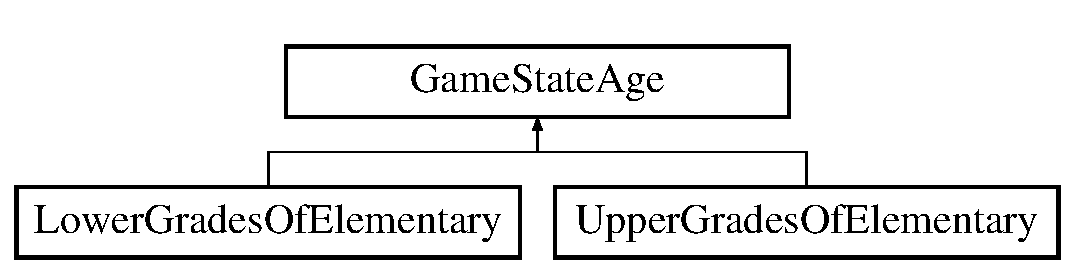
\includegraphics[height=2.000000cm]{class_game_state_age}
\end{center}
\end{figure}
\subsection*{Public メソッド}
\begin{DoxyCompactItemize}
\item 
\hyperlink{class_game_state_age_ae5793d512b139e38125cb1df21905258}{Game\-State\-Age} ()
\item 
virtual void \hyperlink{class_game_state_age_ae2de22cab7976aebb807f228f69309a1}{Set\-Up} ()=0
\item 
virtual \hyperlink{class_game_state_age}{Game\-State\-Age} $\ast$ \hyperlink{class_game_state_age_a21f816167d66266b8c234b40dff4a151}{Next\-Age} ()=0
\item 
virtual std\-::vector$<$ \hyperlink{class_heroine}{Heroine} $>$ \hyperlink{class_game_state_age_a0651ca176cb1e55c4f055aa3907e2165}{Generate\-Enable\-Heroine} ()=0
\item 
virtual std\-::vector$<$ \hyperlink{class_action}{Action} $>$ \hyperlink{class_game_state_age_ac705cfe596fd49e2eec5d8f430f7f848}{Generate\-Enable\-Action} ()=0
\end{DoxyCompactItemize}


\subsection{コンストラクタとデストラクタ}
\hypertarget{class_game_state_age_ae5793d512b139e38125cb1df21905258}{\index{Game\-State\-Age@{Game\-State\-Age}!Game\-State\-Age@{Game\-State\-Age}}
\index{Game\-State\-Age@{Game\-State\-Age}!GameStateAge@{Game\-State\-Age}}
\subsubsection[{Game\-State\-Age}]{\setlength{\rightskip}{0pt plus 5cm}{\bf Game\-State\-Age\-::\-Game\-State\-Age} (
\begin{DoxyParamCaption}
{}
\end{DoxyParamCaption}
)\hspace{0.3cm}{\ttfamily  \mbox{[}inline\mbox{]}}}}\label{class_game_state_age_ae5793d512b139e38125cb1df21905258}


\subsection{関数}
\hypertarget{class_game_state_age_ac705cfe596fd49e2eec5d8f430f7f848}{\index{Game\-State\-Age@{Game\-State\-Age}!Generate\-Enable\-Action@{Generate\-Enable\-Action}}
\index{Generate\-Enable\-Action@{Generate\-Enable\-Action}!GameStateAge@{Game\-State\-Age}}
\subsubsection[{Generate\-Enable\-Action}]{\setlength{\rightskip}{0pt plus 5cm}virtual std\-::vector$<${\bf Action}$>$ {\bf Game\-State\-Age\-::\-Generate\-Enable\-Action} (
\begin{DoxyParamCaption}
{}
\end{DoxyParamCaption}
)\hspace{0.3cm}{\ttfamily  \mbox{[}pure virtual\mbox{]}}}}\label{class_game_state_age_ac705cfe596fd49e2eec5d8f430f7f848}


\hyperlink{class_lower_grades_of_elementary_a868ab761f97d822c3e198d08c0eb1750}{Lower\-Grades\-Of\-Elementary}, と \hyperlink{class_upper_grades_of_elementary_a5ccf297eb998d128f6a01bc210620ed2}{Upper\-Grades\-Of\-Elementary}で実装されています。

\hypertarget{class_game_state_age_a0651ca176cb1e55c4f055aa3907e2165}{\index{Game\-State\-Age@{Game\-State\-Age}!Generate\-Enable\-Heroine@{Generate\-Enable\-Heroine}}
\index{Generate\-Enable\-Heroine@{Generate\-Enable\-Heroine}!GameStateAge@{Game\-State\-Age}}
\subsubsection[{Generate\-Enable\-Heroine}]{\setlength{\rightskip}{0pt plus 5cm}virtual std\-::vector$<${\bf Heroine}$>$ {\bf Game\-State\-Age\-::\-Generate\-Enable\-Heroine} (
\begin{DoxyParamCaption}
{}
\end{DoxyParamCaption}
)\hspace{0.3cm}{\ttfamily  \mbox{[}pure virtual\mbox{]}}}}\label{class_game_state_age_a0651ca176cb1e55c4f055aa3907e2165}


\hyperlink{class_lower_grades_of_elementary_a40b9e24c20d544edadea44a9ebfa1ed9}{Lower\-Grades\-Of\-Elementary}, と \hyperlink{class_upper_grades_of_elementary_a2aff40b541c73636baa75a94bec898ba}{Upper\-Grades\-Of\-Elementary}で実装されています。

\hypertarget{class_game_state_age_a21f816167d66266b8c234b40dff4a151}{\index{Game\-State\-Age@{Game\-State\-Age}!Next\-Age@{Next\-Age}}
\index{Next\-Age@{Next\-Age}!GameStateAge@{Game\-State\-Age}}
\subsubsection[{Next\-Age}]{\setlength{\rightskip}{0pt plus 5cm}virtual {\bf Game\-State\-Age}$\ast$ {\bf Game\-State\-Age\-::\-Next\-Age} (
\begin{DoxyParamCaption}
{}
\end{DoxyParamCaption}
)\hspace{0.3cm}{\ttfamily  \mbox{[}pure virtual\mbox{]}}}}\label{class_game_state_age_a21f816167d66266b8c234b40dff4a151}


\hyperlink{class_lower_grades_of_elementary_a7ba8cff54940dbe8b46c5f0b63874cef}{Lower\-Grades\-Of\-Elementary}, と \hyperlink{class_upper_grades_of_elementary_af772cfb5983b01fdc8b4f5073c6c0e82}{Upper\-Grades\-Of\-Elementary}で実装されています。

\hypertarget{class_game_state_age_ae2de22cab7976aebb807f228f69309a1}{\index{Game\-State\-Age@{Game\-State\-Age}!Set\-Up@{Set\-Up}}
\index{Set\-Up@{Set\-Up}!GameStateAge@{Game\-State\-Age}}
\subsubsection[{Set\-Up}]{\setlength{\rightskip}{0pt plus 5cm}virtual void {\bf Game\-State\-Age\-::\-Set\-Up} (
\begin{DoxyParamCaption}
{}
\end{DoxyParamCaption}
)\hspace{0.3cm}{\ttfamily  \mbox{[}pure virtual\mbox{]}}}}\label{class_game_state_age_ae2de22cab7976aebb807f228f69309a1}


\hyperlink{class_lower_grades_of_elementary_a46665cf9ffd3afe77ddbba1e79def8c6}{Lower\-Grades\-Of\-Elementary}, と \hyperlink{class_upper_grades_of_elementary_a73f1b6ecad28525d60d995765bc504d3}{Upper\-Grades\-Of\-Elementary}で実装されています。



このクラスの説明は次のファイルから生成されました\-:\begin{DoxyCompactItemize}
\item 
Home\-Coming/\hyperlink{_game_state_age_8h}{Game\-State\-Age.\-h}\end{DoxyCompactItemize}

\hypertarget{class_hero}{\section{クラス Hero}
\label{class_hero}\index{Hero@{Hero}}
}


{\ttfamily \#include $<$Hero.\-h$>$}

\subsection*{Public 変数}
\begin{DoxyCompactItemize}
\item 
int \hyperlink{class_hero_a5f9ad5cdca801f5a50a061f4922efd7d}{visual}
\item 
int \hyperlink{class_hero_ab9573020c1704c9f43ab506432940b3b}{intel}
\item 
int \hyperlink{class_hero_a77d140b20f250b02097d3926857ab780}{property}
\item 
int \hyperlink{class_hero_aa5b6f464a1977614dbe6aaa57d18e92a}{human}
\item 
int \hyperlink{class_hero_a3f5b9c15c67f1633720c0697c2defe72}{actpow}
\item 
int \hyperlink{class_hero_a055d2c7f5e0086c118d1abb8536c36a7}{lifepow}
\item 
int \hyperlink{class_hero_ac0e4df7794def10a02d48c1e6dba9c5c}{mindpow}
\item 
int \hyperlink{class_hero_ad4835e0318acceb88198a8a8b11e6a71}{technicpow}
\item 
int \hyperlink{class_hero_a18a85e0df8fb262c9308ab871c2a41e3}{luck}
\item 
int \hyperlink{class_hero_a042bab3291db1aa87c63c99d4ec04afe}{fatalpow}
\item 
int \hyperlink{class_hero_a503facff977509d2d128b1f4fbadfc3d}{talent\-\_\-visual}
\item 
int \hyperlink{class_hero_a059bf1e0f90e5abf88fb7fa649e18f05}{talent\-\_\-intel}
\item 
int \hyperlink{class_hero_a18363568d19a059d64d5864788a04a85}{talent\-\_\-property}
\item 
int \hyperlink{class_hero_af98b757526fa6500d45f39a8a51ee2a8}{talent\-\_\-luck}
\item 
int \hyperlink{class_hero_a38bcfab7d64061895bbdae43693d07ec}{talent\-\_\-lifepow}
\item 
int \hyperlink{class_hero_ad70bb2fa210cd7b1d40f18a894a8b901}{talent\-\_\-technicpow}
\item 
std\-::string \hyperlink{class_hero_a26989c93944866e4f3b9c60cc8f47e0a}{name}
\end{DoxyCompactItemize}


\subsection{変数}
\hypertarget{class_hero_a3f5b9c15c67f1633720c0697c2defe72}{\index{Hero@{Hero}!actpow@{actpow}}
\index{actpow@{actpow}!Hero@{Hero}}
\subsubsection[{actpow}]{\setlength{\rightskip}{0pt plus 5cm}int {\bf Hero\-::actpow}}}\label{class_hero_a3f5b9c15c67f1633720c0697c2defe72}
\hypertarget{class_hero_a042bab3291db1aa87c63c99d4ec04afe}{\index{Hero@{Hero}!fatalpow@{fatalpow}}
\index{fatalpow@{fatalpow}!Hero@{Hero}}
\subsubsection[{fatalpow}]{\setlength{\rightskip}{0pt plus 5cm}int {\bf Hero\-::fatalpow}}}\label{class_hero_a042bab3291db1aa87c63c99d4ec04afe}
\hypertarget{class_hero_aa5b6f464a1977614dbe6aaa57d18e92a}{\index{Hero@{Hero}!human@{human}}
\index{human@{human}!Hero@{Hero}}
\subsubsection[{human}]{\setlength{\rightskip}{0pt plus 5cm}int {\bf Hero\-::human}}}\label{class_hero_aa5b6f464a1977614dbe6aaa57d18e92a}
\hypertarget{class_hero_ab9573020c1704c9f43ab506432940b3b}{\index{Hero@{Hero}!intel@{intel}}
\index{intel@{intel}!Hero@{Hero}}
\subsubsection[{intel}]{\setlength{\rightskip}{0pt plus 5cm}int {\bf Hero\-::intel}}}\label{class_hero_ab9573020c1704c9f43ab506432940b3b}
\hypertarget{class_hero_a055d2c7f5e0086c118d1abb8536c36a7}{\index{Hero@{Hero}!lifepow@{lifepow}}
\index{lifepow@{lifepow}!Hero@{Hero}}
\subsubsection[{lifepow}]{\setlength{\rightskip}{0pt plus 5cm}int {\bf Hero\-::lifepow}}}\label{class_hero_a055d2c7f5e0086c118d1abb8536c36a7}
\hypertarget{class_hero_a18a85e0df8fb262c9308ab871c2a41e3}{\index{Hero@{Hero}!luck@{luck}}
\index{luck@{luck}!Hero@{Hero}}
\subsubsection[{luck}]{\setlength{\rightskip}{0pt plus 5cm}int {\bf Hero\-::luck}}}\label{class_hero_a18a85e0df8fb262c9308ab871c2a41e3}
\hypertarget{class_hero_ac0e4df7794def10a02d48c1e6dba9c5c}{\index{Hero@{Hero}!mindpow@{mindpow}}
\index{mindpow@{mindpow}!Hero@{Hero}}
\subsubsection[{mindpow}]{\setlength{\rightskip}{0pt plus 5cm}int {\bf Hero\-::mindpow}}}\label{class_hero_ac0e4df7794def10a02d48c1e6dba9c5c}
\hypertarget{class_hero_a26989c93944866e4f3b9c60cc8f47e0a}{\index{Hero@{Hero}!name@{name}}
\index{name@{name}!Hero@{Hero}}
\subsubsection[{name}]{\setlength{\rightskip}{0pt plus 5cm}std\-::string {\bf Hero\-::name}}}\label{class_hero_a26989c93944866e4f3b9c60cc8f47e0a}
\hypertarget{class_hero_a77d140b20f250b02097d3926857ab780}{\index{Hero@{Hero}!property@{property}}
\index{property@{property}!Hero@{Hero}}
\subsubsection[{property}]{\setlength{\rightskip}{0pt plus 5cm}int {\bf Hero\-::property}}}\label{class_hero_a77d140b20f250b02097d3926857ab780}
\hypertarget{class_hero_a059bf1e0f90e5abf88fb7fa649e18f05}{\index{Hero@{Hero}!talent\-\_\-intel@{talent\-\_\-intel}}
\index{talent\-\_\-intel@{talent\-\_\-intel}!Hero@{Hero}}
\subsubsection[{talent\-\_\-intel}]{\setlength{\rightskip}{0pt plus 5cm}int {\bf Hero\-::talent\-\_\-intel}}}\label{class_hero_a059bf1e0f90e5abf88fb7fa649e18f05}
\hypertarget{class_hero_a38bcfab7d64061895bbdae43693d07ec}{\index{Hero@{Hero}!talent\-\_\-lifepow@{talent\-\_\-lifepow}}
\index{talent\-\_\-lifepow@{talent\-\_\-lifepow}!Hero@{Hero}}
\subsubsection[{talent\-\_\-lifepow}]{\setlength{\rightskip}{0pt plus 5cm}int {\bf Hero\-::talent\-\_\-lifepow}}}\label{class_hero_a38bcfab7d64061895bbdae43693d07ec}
\hypertarget{class_hero_af98b757526fa6500d45f39a8a51ee2a8}{\index{Hero@{Hero}!talent\-\_\-luck@{talent\-\_\-luck}}
\index{talent\-\_\-luck@{talent\-\_\-luck}!Hero@{Hero}}
\subsubsection[{talent\-\_\-luck}]{\setlength{\rightskip}{0pt plus 5cm}int {\bf Hero\-::talent\-\_\-luck}}}\label{class_hero_af98b757526fa6500d45f39a8a51ee2a8}
\hypertarget{class_hero_a18363568d19a059d64d5864788a04a85}{\index{Hero@{Hero}!talent\-\_\-property@{talent\-\_\-property}}
\index{talent\-\_\-property@{talent\-\_\-property}!Hero@{Hero}}
\subsubsection[{talent\-\_\-property}]{\setlength{\rightskip}{0pt plus 5cm}int {\bf Hero\-::talent\-\_\-property}}}\label{class_hero_a18363568d19a059d64d5864788a04a85}
\hypertarget{class_hero_ad70bb2fa210cd7b1d40f18a894a8b901}{\index{Hero@{Hero}!talent\-\_\-technicpow@{talent\-\_\-technicpow}}
\index{talent\-\_\-technicpow@{talent\-\_\-technicpow}!Hero@{Hero}}
\subsubsection[{talent\-\_\-technicpow}]{\setlength{\rightskip}{0pt plus 5cm}int {\bf Hero\-::talent\-\_\-technicpow}}}\label{class_hero_ad70bb2fa210cd7b1d40f18a894a8b901}
\hypertarget{class_hero_a503facff977509d2d128b1f4fbadfc3d}{\index{Hero@{Hero}!talent\-\_\-visual@{talent\-\_\-visual}}
\index{talent\-\_\-visual@{talent\-\_\-visual}!Hero@{Hero}}
\subsubsection[{talent\-\_\-visual}]{\setlength{\rightskip}{0pt plus 5cm}int {\bf Hero\-::talent\-\_\-visual}}}\label{class_hero_a503facff977509d2d128b1f4fbadfc3d}
\hypertarget{class_hero_ad4835e0318acceb88198a8a8b11e6a71}{\index{Hero@{Hero}!technicpow@{technicpow}}
\index{technicpow@{technicpow}!Hero@{Hero}}
\subsubsection[{technicpow}]{\setlength{\rightskip}{0pt plus 5cm}int {\bf Hero\-::technicpow}}}\label{class_hero_ad4835e0318acceb88198a8a8b11e6a71}
\hypertarget{class_hero_a5f9ad5cdca801f5a50a061f4922efd7d}{\index{Hero@{Hero}!visual@{visual}}
\index{visual@{visual}!Hero@{Hero}}
\subsubsection[{visual}]{\setlength{\rightskip}{0pt plus 5cm}int {\bf Hero\-::visual}}}\label{class_hero_a5f9ad5cdca801f5a50a061f4922efd7d}


このクラスの説明は次のファイルから生成されました\-:\begin{DoxyCompactItemize}
\item 
Home\-Coming/\hyperlink{_hero_8h}{Hero.\-h}\end{DoxyCompactItemize}

\hypertarget{class_heroine}{\section{クラス Heroine}
\label{class_heroine}\index{Heroine@{Heroine}}
}


{\ttfamily \#include $<$Heroine.\-h$>$}

\subsection*{Public 変数}
\begin{DoxyCompactItemize}
\item 
std\-::string \hyperlink{class_heroine_a0ab7a4e9b216f96c5e8e8248af55e71a}{name}
\item 
int \hyperlink{class_heroine_a2e514d4fc23f767db26d784c68b873aa}{visual}
\item 
int \hyperlink{class_heroine_a085a99674b147d11ea0485dd92ff015e}{intel}
\item 
int \hyperlink{class_heroine_a17ef1aa15d58ef8eed9a319d59ee270f}{property}
\item 
int \hyperlink{class_heroine_a0fa65600a12799447189c09a0bee7b3e}{human}
\item 
int \hyperlink{class_heroine_ac61fab4be574f24f4acba98ffb378659}{actpow}
\item 
int \hyperlink{class_heroine_ae345b69491b13d0ff434fd9660e6d512}{lifepow}
\item 
int \hyperlink{class_heroine_a8d7c5cbfa1d9fafef76104f66af22f9c}{mindpow}
\item 
int \hyperlink{class_heroine_a7456ab0e6a903a4463791122bd3f2d77}{technicpow}
\item 
int \hyperlink{class_heroine_a23fc3ab3592baaac8b2a4bd3a8e35d01}{luck}
\item 
std\-::vector$<$ \hyperlink{class_heroine_attr}{Heroine\-Attr} $>$ \hyperlink{class_heroine_a9ffecfedbbc121692855ca1549cfe4b5}{attrs}
\item 
int \hyperlink{class_heroine_a36a37961c5006658137fe5e7de17282a}{schoolid}
\item 
int \hyperlink{class_heroine_ae4b64050de16a8057995ad6dc16ebcad}{age}
\item 
bool \hyperlink{class_heroine_a076bc8f1ba22d3214059214b6f94b255}{appear\-O\-K}
\end{DoxyCompactItemize}


\subsection{変数}
\hypertarget{class_heroine_ac61fab4be574f24f4acba98ffb378659}{\index{Heroine@{Heroine}!actpow@{actpow}}
\index{actpow@{actpow}!Heroine@{Heroine}}
\subsubsection[{actpow}]{\setlength{\rightskip}{0pt plus 5cm}int {\bf Heroine\-::actpow}}}\label{class_heroine_ac61fab4be574f24f4acba98ffb378659}
\hypertarget{class_heroine_ae4b64050de16a8057995ad6dc16ebcad}{\index{Heroine@{Heroine}!age@{age}}
\index{age@{age}!Heroine@{Heroine}}
\subsubsection[{age}]{\setlength{\rightskip}{0pt plus 5cm}int {\bf Heroine\-::age}}}\label{class_heroine_ae4b64050de16a8057995ad6dc16ebcad}
\hypertarget{class_heroine_a076bc8f1ba22d3214059214b6f94b255}{\index{Heroine@{Heroine}!appear\-O\-K@{appear\-O\-K}}
\index{appear\-O\-K@{appear\-O\-K}!Heroine@{Heroine}}
\subsubsection[{appear\-O\-K}]{\setlength{\rightskip}{0pt plus 5cm}bool {\bf Heroine\-::appear\-O\-K}}}\label{class_heroine_a076bc8f1ba22d3214059214b6f94b255}
\hypertarget{class_heroine_a9ffecfedbbc121692855ca1549cfe4b5}{\index{Heroine@{Heroine}!attrs@{attrs}}
\index{attrs@{attrs}!Heroine@{Heroine}}
\subsubsection[{attrs}]{\setlength{\rightskip}{0pt plus 5cm}std\-::vector$<${\bf Heroine\-Attr}$>$ {\bf Heroine\-::attrs}}}\label{class_heroine_a9ffecfedbbc121692855ca1549cfe4b5}
\hypertarget{class_heroine_a0fa65600a12799447189c09a0bee7b3e}{\index{Heroine@{Heroine}!human@{human}}
\index{human@{human}!Heroine@{Heroine}}
\subsubsection[{human}]{\setlength{\rightskip}{0pt plus 5cm}int {\bf Heroine\-::human}}}\label{class_heroine_a0fa65600a12799447189c09a0bee7b3e}
\hypertarget{class_heroine_a085a99674b147d11ea0485dd92ff015e}{\index{Heroine@{Heroine}!intel@{intel}}
\index{intel@{intel}!Heroine@{Heroine}}
\subsubsection[{intel}]{\setlength{\rightskip}{0pt plus 5cm}int {\bf Heroine\-::intel}}}\label{class_heroine_a085a99674b147d11ea0485dd92ff015e}
\hypertarget{class_heroine_ae345b69491b13d0ff434fd9660e6d512}{\index{Heroine@{Heroine}!lifepow@{lifepow}}
\index{lifepow@{lifepow}!Heroine@{Heroine}}
\subsubsection[{lifepow}]{\setlength{\rightskip}{0pt plus 5cm}int {\bf Heroine\-::lifepow}}}\label{class_heroine_ae345b69491b13d0ff434fd9660e6d512}
\hypertarget{class_heroine_a23fc3ab3592baaac8b2a4bd3a8e35d01}{\index{Heroine@{Heroine}!luck@{luck}}
\index{luck@{luck}!Heroine@{Heroine}}
\subsubsection[{luck}]{\setlength{\rightskip}{0pt plus 5cm}int {\bf Heroine\-::luck}}}\label{class_heroine_a23fc3ab3592baaac8b2a4bd3a8e35d01}
\hypertarget{class_heroine_a8d7c5cbfa1d9fafef76104f66af22f9c}{\index{Heroine@{Heroine}!mindpow@{mindpow}}
\index{mindpow@{mindpow}!Heroine@{Heroine}}
\subsubsection[{mindpow}]{\setlength{\rightskip}{0pt plus 5cm}int {\bf Heroine\-::mindpow}}}\label{class_heroine_a8d7c5cbfa1d9fafef76104f66af22f9c}
\hypertarget{class_heroine_a0ab7a4e9b216f96c5e8e8248af55e71a}{\index{Heroine@{Heroine}!name@{name}}
\index{name@{name}!Heroine@{Heroine}}
\subsubsection[{name}]{\setlength{\rightskip}{0pt plus 5cm}std\-::string {\bf Heroine\-::name}}}\label{class_heroine_a0ab7a4e9b216f96c5e8e8248af55e71a}
\hypertarget{class_heroine_a17ef1aa15d58ef8eed9a319d59ee270f}{\index{Heroine@{Heroine}!property@{property}}
\index{property@{property}!Heroine@{Heroine}}
\subsubsection[{property}]{\setlength{\rightskip}{0pt plus 5cm}int {\bf Heroine\-::property}}}\label{class_heroine_a17ef1aa15d58ef8eed9a319d59ee270f}
\hypertarget{class_heroine_a36a37961c5006658137fe5e7de17282a}{\index{Heroine@{Heroine}!schoolid@{schoolid}}
\index{schoolid@{schoolid}!Heroine@{Heroine}}
\subsubsection[{schoolid}]{\setlength{\rightskip}{0pt plus 5cm}int {\bf Heroine\-::schoolid}}}\label{class_heroine_a36a37961c5006658137fe5e7de17282a}
\hypertarget{class_heroine_a7456ab0e6a903a4463791122bd3f2d77}{\index{Heroine@{Heroine}!technicpow@{technicpow}}
\index{technicpow@{technicpow}!Heroine@{Heroine}}
\subsubsection[{technicpow}]{\setlength{\rightskip}{0pt plus 5cm}int {\bf Heroine\-::technicpow}}}\label{class_heroine_a7456ab0e6a903a4463791122bd3f2d77}
\hypertarget{class_heroine_a2e514d4fc23f767db26d784c68b873aa}{\index{Heroine@{Heroine}!visual@{visual}}
\index{visual@{visual}!Heroine@{Heroine}}
\subsubsection[{visual}]{\setlength{\rightskip}{0pt plus 5cm}int {\bf Heroine\-::visual}}}\label{class_heroine_a2e514d4fc23f767db26d784c68b873aa}


このクラスの説明は次のファイルから生成されました\-:\begin{DoxyCompactItemize}
\item 
Home\-Coming/\hyperlink{_heroine_8h}{Heroine.\-h}\end{DoxyCompactItemize}

\hypertarget{class_heroine_attr}{\section{クラス Heroine\-Attr}
\label{class_heroine_attr}\index{Heroine\-Attr@{Heroine\-Attr}}
}


{\ttfamily \#include $<$Heroine.\-h$>$}



このクラスの説明は次のファイルから生成されました\-:\begin{DoxyCompactItemize}
\item 
Home\-Coming/\hyperlink{_heroine_8h}{Heroine.\-h}\end{DoxyCompactItemize}

\hypertarget{interface_heroine_table_data}{\section{クラス Heroine\-Table\-Data}
\label{interface_heroine_table_data}\index{Heroine\-Table\-Data@{Heroine\-Table\-Data}}
}


{\ttfamily \#import $<$Heroine\-Table\-Data.\-h$>$}

\subsection*{Public メソッド}
\begin{DoxyCompactItemize}
\item 
(id) -\/ \hyperlink{interface_heroine_table_data_a151650b2c966a6158a9faacf88ab6665}{init\-With\-Heroine\-:}
\end{DoxyCompactItemize}
\subsection*{Protected 変数}
\begin{DoxyCompactItemize}
\item 
\hyperlink{class_heroine}{Heroine} \hyperlink{interface_heroine_table_data_a015f516b3cb364ce0241d41c916cb635}{data}
\end{DoxyCompactItemize}
\subsection*{プロパティ}
\begin{DoxyCompactItemize}
\item 
N\-S\-String $\ast$ \hyperlink{interface_heroine_table_data_aad898ba45388237fc9d124cff49e7ca6}{display\-\_\-name}
\end{DoxyCompactItemize}


\subsection{関数}
\hypertarget{interface_heroine_table_data_a151650b2c966a6158a9faacf88ab6665}{\index{Heroine\-Table\-Data@{Heroine\-Table\-Data}!init\-With\-Heroine\-:@{init\-With\-Heroine\-:}}
\index{init\-With\-Heroine\-:@{init\-With\-Heroine\-:}!HeroineTableData@{Heroine\-Table\-Data}}
\subsubsection[{init\-With\-Heroine\-:}]{\setlength{\rightskip}{0pt plus 5cm}-\/ (id) {\bf init\-With\-Heroine\-:} 
\begin{DoxyParamCaption}
\item[{({\bf Heroine})}]{heroine}
\end{DoxyParamCaption}
}}\label{interface_heroine_table_data_a151650b2c966a6158a9faacf88ab6665}


\subsection{変数}
\hypertarget{interface_heroine_table_data_a015f516b3cb364ce0241d41c916cb635}{\index{Heroine\-Table\-Data@{Heroine\-Table\-Data}!data@{data}}
\index{data@{data}!HeroineTableData@{Heroine\-Table\-Data}}
\subsubsection[{data}]{\setlength{\rightskip}{0pt plus 5cm}-\/ ({\bf Heroine}) {\bf data}\hspace{0.3cm}{\ttfamily  \mbox{[}protected\mbox{]}}}}\label{interface_heroine_table_data_a015f516b3cb364ce0241d41c916cb635}


\subsection{プロパティ}
\hypertarget{interface_heroine_table_data_aad898ba45388237fc9d124cff49e7ca6}{\index{Heroine\-Table\-Data@{Heroine\-Table\-Data}!display\-\_\-name@{display\-\_\-name}}
\index{display\-\_\-name@{display\-\_\-name}!HeroineTableData@{Heroine\-Table\-Data}}
\subsubsection[{display\-\_\-name}]{\setlength{\rightskip}{0pt plus 5cm}-\/ (N\-S\-String $\ast$) {\bf display\-\_\-name}\hspace{0.3cm}{\ttfamily  \mbox{[}read, write, retain\mbox{]}}}}\label{interface_heroine_table_data_aad898ba45388237fc9d124cff49e7ca6}


このクラスの説明は次のファイルから生成されました\-:\begin{DoxyCompactItemize}
\item 
Home\-Coming/\hyperlink{_heroine_table_data_8h}{Heroine\-Table\-Data.\-h}\item 
Home\-Coming/\hyperlink{_heroine_table_data_8m}{Heroine\-Table\-Data.\-m}\end{DoxyCompactItemize}

\hypertarget{class_lower_grades_of_elementary}{\section{クラス Lower\-Grades\-Of\-Elementary}
\label{class_lower_grades_of_elementary}\index{Lower\-Grades\-Of\-Elementary@{Lower\-Grades\-Of\-Elementary}}
}


{\ttfamily \#include $<$Lower\-Grades\-Of\-Elementary.\-h$>$}

Lower\-Grades\-Of\-Elementaryに対する継承グラフ\begin{figure}[H]
\begin{center}
\leavevmode
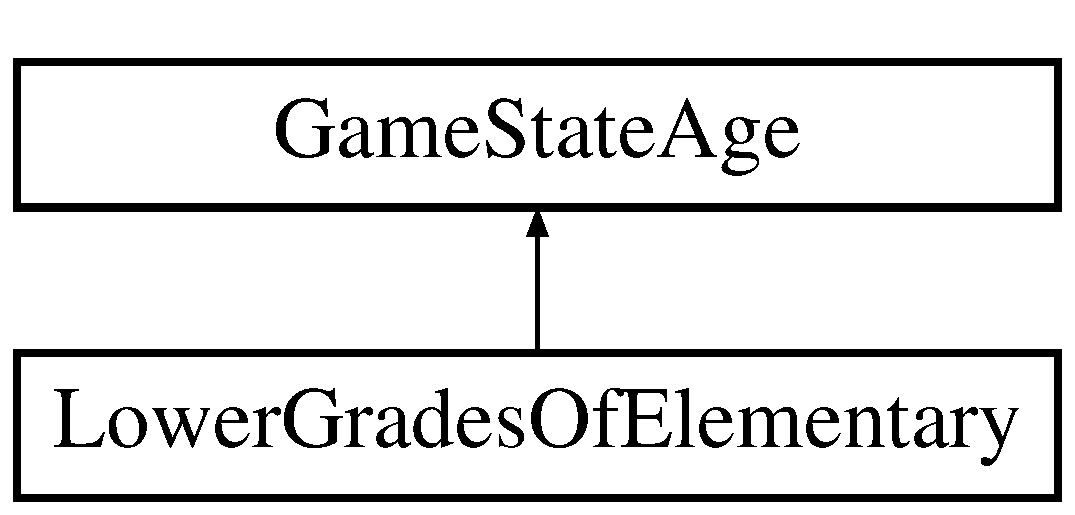
\includegraphics[height=2.000000cm]{class_lower_grades_of_elementary}
\end{center}
\end{figure}
\subsection*{Public メソッド}
\begin{DoxyCompactItemize}
\item 
\hyperlink{class_lower_grades_of_elementary_a4c5267135474bafa05293e7c9fcda2cb}{Lower\-Grades\-Of\-Elementary} ()
\item 
void \hyperlink{class_lower_grades_of_elementary_a46665cf9ffd3afe77ddbba1e79def8c6}{Set\-Up} ()
\item 
\hyperlink{class_game_state_age}{Game\-State\-Age} $\ast$ \hyperlink{class_lower_grades_of_elementary_a7ba8cff54940dbe8b46c5f0b63874cef}{Next\-Age} ()
\item 
std\-::vector$<$ \hyperlink{class_heroine}{Heroine} $>$ \hyperlink{class_lower_grades_of_elementary_a40b9e24c20d544edadea44a9ebfa1ed9}{Generate\-Enable\-Heroine} ()
\item 
std\-::vector$<$ \hyperlink{class_action}{Action} $>$ \hyperlink{class_lower_grades_of_elementary_a868ab761f97d822c3e198d08c0eb1750}{Generate\-Enable\-Action} ()
\end{DoxyCompactItemize}


\subsection{コンストラクタとデストラクタ}
\hypertarget{class_lower_grades_of_elementary_a4c5267135474bafa05293e7c9fcda2cb}{\index{Lower\-Grades\-Of\-Elementary@{Lower\-Grades\-Of\-Elementary}!Lower\-Grades\-Of\-Elementary@{Lower\-Grades\-Of\-Elementary}}
\index{Lower\-Grades\-Of\-Elementary@{Lower\-Grades\-Of\-Elementary}!LowerGradesOfElementary@{Lower\-Grades\-Of\-Elementary}}
\subsubsection[{Lower\-Grades\-Of\-Elementary}]{\setlength{\rightskip}{0pt plus 5cm}{\bf Lower\-Grades\-Of\-Elementary\-::\-Lower\-Grades\-Of\-Elementary} (
\begin{DoxyParamCaption}
{}
\end{DoxyParamCaption}
)}}\label{class_lower_grades_of_elementary_a4c5267135474bafa05293e7c9fcda2cb}


\subsection{関数}
\hypertarget{class_lower_grades_of_elementary_a868ab761f97d822c3e198d08c0eb1750}{\index{Lower\-Grades\-Of\-Elementary@{Lower\-Grades\-Of\-Elementary}!Generate\-Enable\-Action@{Generate\-Enable\-Action}}
\index{Generate\-Enable\-Action@{Generate\-Enable\-Action}!LowerGradesOfElementary@{Lower\-Grades\-Of\-Elementary}}
\subsubsection[{Generate\-Enable\-Action}]{\setlength{\rightskip}{0pt plus 5cm}vector$<$ {\bf Action} $>$ {\bf Lower\-Grades\-Of\-Elementary\-::\-Generate\-Enable\-Action} (
\begin{DoxyParamCaption}
{}
\end{DoxyParamCaption}
)\hspace{0.3cm}{\ttfamily  \mbox{[}virtual\mbox{]}}}}\label{class_lower_grades_of_elementary_a868ab761f97d822c3e198d08c0eb1750}


\hyperlink{class_game_state_age_ac705cfe596fd49e2eec5d8f430f7f848}{Game\-State\-Age}を実装しています。

\hypertarget{class_lower_grades_of_elementary_a40b9e24c20d544edadea44a9ebfa1ed9}{\index{Lower\-Grades\-Of\-Elementary@{Lower\-Grades\-Of\-Elementary}!Generate\-Enable\-Heroine@{Generate\-Enable\-Heroine}}
\index{Generate\-Enable\-Heroine@{Generate\-Enable\-Heroine}!LowerGradesOfElementary@{Lower\-Grades\-Of\-Elementary}}
\subsubsection[{Generate\-Enable\-Heroine}]{\setlength{\rightskip}{0pt plus 5cm}vector$<$ {\bf Heroine} $>$ {\bf Lower\-Grades\-Of\-Elementary\-::\-Generate\-Enable\-Heroine} (
\begin{DoxyParamCaption}
{}
\end{DoxyParamCaption}
)\hspace{0.3cm}{\ttfamily  \mbox{[}virtual\mbox{]}}}}\label{class_lower_grades_of_elementary_a40b9e24c20d544edadea44a9ebfa1ed9}


\hyperlink{class_game_state_age_a0651ca176cb1e55c4f055aa3907e2165}{Game\-State\-Age}を実装しています。

\hypertarget{class_lower_grades_of_elementary_a7ba8cff54940dbe8b46c5f0b63874cef}{\index{Lower\-Grades\-Of\-Elementary@{Lower\-Grades\-Of\-Elementary}!Next\-Age@{Next\-Age}}
\index{Next\-Age@{Next\-Age}!LowerGradesOfElementary@{Lower\-Grades\-Of\-Elementary}}
\subsubsection[{Next\-Age}]{\setlength{\rightskip}{0pt plus 5cm}{\bf Game\-State\-Age} $\ast$ {\bf Lower\-Grades\-Of\-Elementary\-::\-Next\-Age} (
\begin{DoxyParamCaption}
{}
\end{DoxyParamCaption}
)\hspace{0.3cm}{\ttfamily  \mbox{[}virtual\mbox{]}}}}\label{class_lower_grades_of_elementary_a7ba8cff54940dbe8b46c5f0b63874cef}


\hyperlink{class_game_state_age_a21f816167d66266b8c234b40dff4a151}{Game\-State\-Age}を実装しています。

\hypertarget{class_lower_grades_of_elementary_a46665cf9ffd3afe77ddbba1e79def8c6}{\index{Lower\-Grades\-Of\-Elementary@{Lower\-Grades\-Of\-Elementary}!Set\-Up@{Set\-Up}}
\index{Set\-Up@{Set\-Up}!LowerGradesOfElementary@{Lower\-Grades\-Of\-Elementary}}
\subsubsection[{Set\-Up}]{\setlength{\rightskip}{0pt plus 5cm}void {\bf Lower\-Grades\-Of\-Elementary\-::\-Set\-Up} (
\begin{DoxyParamCaption}
{}
\end{DoxyParamCaption}
)\hspace{0.3cm}{\ttfamily  \mbox{[}virtual\mbox{]}}}}\label{class_lower_grades_of_elementary_a46665cf9ffd3afe77ddbba1e79def8c6}


\hyperlink{class_game_state_age_ae2de22cab7976aebb807f228f69309a1}{Game\-State\-Age}を実装しています。



このクラスの説明は次のファイルから生成されました\-:\begin{DoxyCompactItemize}
\item 
Home\-Coming/\hyperlink{_lower_grades_of_elementary_8h}{Lower\-Grades\-Of\-Elementary.\-h}\item 
Home\-Coming/\hyperlink{_lower_grades_of_elementary_8cpp}{Lower\-Grades\-Of\-Elementary.\-cpp}\end{DoxyCompactItemize}

\hypertarget{struct_range_number}{\section{構造体 Range\-Number}
\label{struct_range_number}\index{Range\-Number@{Range\-Number}}
}


{\ttfamily \#include $<$Utility.\-h$>$}

\subsection*{Public メソッド}
\begin{DoxyCompactItemize}
\item 
\hyperlink{struct_range_number_ae65f83dd5c79b86a781d594e30edac17}{Range\-Number} (int lb, int ub)
\item 
\hyperlink{struct_range_number_a72c9b0f36cfb6c1b99d692daafafddf1}{Range\-Number} ()
\end{DoxyCompactItemize}
\subsection*{Public 変数}
\begin{DoxyCompactItemize}
\item 
int \hyperlink{struct_range_number_a0ba35a5ec8d4c1184344e4e90f1d7c6b}{low}
\item 
int \hyperlink{struct_range_number_afdc3b20ea90fa3c85c7a581c0cce3236}{up}
\end{DoxyCompactItemize}


\subsection{コンストラクタとデストラクタ}
\hypertarget{struct_range_number_ae65f83dd5c79b86a781d594e30edac17}{\index{Range\-Number@{Range\-Number}!Range\-Number@{Range\-Number}}
\index{Range\-Number@{Range\-Number}!RangeNumber@{Range\-Number}}
\subsubsection[{Range\-Number}]{\setlength{\rightskip}{0pt plus 5cm}{\bf Range\-Number\-::\-Range\-Number} (
\begin{DoxyParamCaption}
\item[{int}]{lb, }
\item[{int}]{ub}
\end{DoxyParamCaption}
)\hspace{0.3cm}{\ttfamily  \mbox{[}inline\mbox{]}}}}\label{struct_range_number_ae65f83dd5c79b86a781d594e30edac17}
\hypertarget{struct_range_number_a72c9b0f36cfb6c1b99d692daafafddf1}{\index{Range\-Number@{Range\-Number}!Range\-Number@{Range\-Number}}
\index{Range\-Number@{Range\-Number}!RangeNumber@{Range\-Number}}
\subsubsection[{Range\-Number}]{\setlength{\rightskip}{0pt plus 5cm}{\bf Range\-Number\-::\-Range\-Number} (
\begin{DoxyParamCaption}
{}
\end{DoxyParamCaption}
)\hspace{0.3cm}{\ttfamily  \mbox{[}inline\mbox{]}}}}\label{struct_range_number_a72c9b0f36cfb6c1b99d692daafafddf1}


\subsection{変数}
\hypertarget{struct_range_number_a0ba35a5ec8d4c1184344e4e90f1d7c6b}{\index{Range\-Number@{Range\-Number}!low@{low}}
\index{low@{low}!RangeNumber@{Range\-Number}}
\subsubsection[{low}]{\setlength{\rightskip}{0pt plus 5cm}int {\bf Range\-Number\-::low}}}\label{struct_range_number_a0ba35a5ec8d4c1184344e4e90f1d7c6b}
\hypertarget{struct_range_number_afdc3b20ea90fa3c85c7a581c0cce3236}{\index{Range\-Number@{Range\-Number}!up@{up}}
\index{up@{up}!RangeNumber@{Range\-Number}}
\subsubsection[{up}]{\setlength{\rightskip}{0pt plus 5cm}int {\bf Range\-Number\-::up}}}\label{struct_range_number_afdc3b20ea90fa3c85c7a581c0cce3236}


この構造体の説明は次のファイルから生成されました\-:\begin{DoxyCompactItemize}
\item 
Home\-Coming/\hyperlink{_utility_8h}{Utility.\-h}\end{DoxyCompactItemize}

\hypertarget{class_school}{\section{クラス School}
\label{class_school}\index{School@{School}}
}


{\ttfamily \#include $<$School.\-h$>$}



このクラスの説明は次のファイルから生成されました\-:\begin{DoxyCompactItemize}
\item 
Home\-Coming/\hyperlink{_school_8h}{School.\-h}\end{DoxyCompactItemize}

\hypertarget{class_story}{\section{クラス Story}
\label{class_story}\index{Story@{Story}}
}


{\ttfamily \#include $<$Story.\-hpp$>$}

\subsection*{Public メソッド}
\begin{DoxyCompactItemize}
\item 
std\-::string \hyperlink{class_story_aad0be22d7fb9e20aa06eb671fac6a2e9}{get\-Text} (int idx)
\item 
std\-::string \hyperlink{class_story_a7ec46e72ac2dd44451178781f6b78ef2}{get\-Image\-Path} (int idx)
\end{DoxyCompactItemize}
\subsection*{Static Public メソッド}
\begin{DoxyCompactItemize}
\item 
static \hyperlink{class_story}{Story} \hyperlink{class_story_a5d9613a28e0888cd74a5e309c4d3ffbf}{load} (const char $\ast$path)
\end{DoxyCompactItemize}


\subsection{関数}
\hypertarget{class_story_a7ec46e72ac2dd44451178781f6b78ef2}{\index{Story@{Story}!get\-Image\-Path@{get\-Image\-Path}}
\index{get\-Image\-Path@{get\-Image\-Path}!Story@{Story}}
\subsubsection[{get\-Image\-Path}]{\setlength{\rightskip}{0pt plus 5cm}std\-::string {\bf Story\-::get\-Image\-Path} (
\begin{DoxyParamCaption}
\item[{int}]{idx}
\end{DoxyParamCaption}
)}}\label{class_story_a7ec46e72ac2dd44451178781f6b78ef2}
\hypertarget{class_story_aad0be22d7fb9e20aa06eb671fac6a2e9}{\index{Story@{Story}!get\-Text@{get\-Text}}
\index{get\-Text@{get\-Text}!Story@{Story}}
\subsubsection[{get\-Text}]{\setlength{\rightskip}{0pt plus 5cm}std\-::string {\bf Story\-::get\-Text} (
\begin{DoxyParamCaption}
\item[{int}]{idx}
\end{DoxyParamCaption}
)}}\label{class_story_aad0be22d7fb9e20aa06eb671fac6a2e9}
\hypertarget{class_story_a5d9613a28e0888cd74a5e309c4d3ffbf}{\index{Story@{Story}!load@{load}}
\index{load@{load}!Story@{Story}}
\subsubsection[{load}]{\setlength{\rightskip}{0pt plus 5cm}static {\bf Story} {\bf Story\-::load} (
\begin{DoxyParamCaption}
\item[{const char $\ast$}]{path}
\end{DoxyParamCaption}
)\hspace{0.3cm}{\ttfamily  \mbox{[}static\mbox{]}}}}\label{class_story_a5d9613a28e0888cd74a5e309c4d3ffbf}


このクラスの説明は次のファイルから生成されました\-:\begin{DoxyCompactItemize}
\item 
Home\-Coming/\hyperlink{_story_8hpp}{Story.\-hpp}\end{DoxyCompactItemize}

\hypertarget{interface_story_view}{\section{クラス Story\-View}
\label{interface_story_view}\index{Story\-View@{Story\-View}}
}


{\ttfamily \#import $<$Story\-View.\-h$>$}

\subsection*{Public メソッド}
\begin{DoxyCompactItemize}
\item 
(void) -\/ \hyperlink{interface_story_view_a39df58581273ccc9df0aec0e22c05c78}{\-\_\-turn\-Over\-Pages\-:}
\end{DoxyCompactItemize}
\subsection*{Protected 変数}
\begin{DoxyCompactItemize}
\item 
int \hyperlink{interface_story_view_abccb39685ba306e97ffea7681c23fceb}{\-\_\-story\-Index}
\item 
\hyperlink{class_story}{Story} $\ast$ \hyperlink{interface_story_view_a6d301e4a4e0465419eb6419c9c38db37}{story}
\end{DoxyCompactItemize}
\subsection*{プロパティ}
\begin{DoxyCompactItemize}
\item 
int \hyperlink{interface_story_view_a6f4fd6e85a6e6fcc6911ea70f1d6da28}{story\-Index}
\item 
id \hyperlink{interface_story_view_ae5170731a3cb2f2a923b896ce5620b94}{target}
\item 
S\-E\-L \hyperlink{interface_story_view_a5b484336016f06b152943becab7e1089}{action}
\end{DoxyCompactItemize}


\subsection{関数}
\hypertarget{interface_story_view_a39df58581273ccc9df0aec0e22c05c78}{\index{Story\-View@{Story\-View}!\-\_\-turn\-Over\-Pages\-:@{\-\_\-turn\-Over\-Pages\-:}}
\index{\-\_\-turn\-Over\-Pages\-:@{\-\_\-turn\-Over\-Pages\-:}!StoryView@{Story\-View}}
\subsubsection[{\-\_\-turn\-Over\-Pages\-:}]{\setlength{\rightskip}{0pt plus 5cm}-\/ (void) {\bf \-\_\-turn\-Over\-Pages\-:} 
\begin{DoxyParamCaption}
\item[{(N\-S\-Event $\ast$)}]{the\-Event}
\end{DoxyParamCaption}
}}\label{interface_story_view_a39df58581273ccc9df0aec0e22c05c78}


\subsection{変数}
\hypertarget{interface_story_view_abccb39685ba306e97ffea7681c23fceb}{\index{Story\-View@{Story\-View}!\-\_\-story\-Index@{\-\_\-story\-Index}}
\index{\-\_\-story\-Index@{\-\_\-story\-Index}!StoryView@{Story\-View}}
\subsubsection[{\-\_\-story\-Index}]{\setlength{\rightskip}{0pt plus 5cm}-\/ (int) {\bf \-\_\-story\-Index}\hspace{0.3cm}{\ttfamily  \mbox{[}protected\mbox{]}}}}\label{interface_story_view_abccb39685ba306e97ffea7681c23fceb}
\hypertarget{interface_story_view_a6d301e4a4e0465419eb6419c9c38db37}{\index{Story\-View@{Story\-View}!story@{story}}
\index{story@{story}!StoryView@{Story\-View}}
\subsubsection[{story}]{\setlength{\rightskip}{0pt plus 5cm}-\/ ({\bf Story}$\ast$) {\bf story}\hspace{0.3cm}{\ttfamily  \mbox{[}protected\mbox{]}}}}\label{interface_story_view_a6d301e4a4e0465419eb6419c9c38db37}


\subsection{プロパティ}
\hypertarget{interface_story_view_a5b484336016f06b152943becab7e1089}{\index{Story\-View@{Story\-View}!action@{action}}
\index{action@{action}!StoryView@{Story\-View}}
\subsubsection[{action}]{\setlength{\rightskip}{0pt plus 5cm}-\/ (S\-E\-L) {\bf action}\hspace{0.3cm}{\ttfamily  \mbox{[}read, write, assign\mbox{]}}}}\label{interface_story_view_a5b484336016f06b152943becab7e1089}
\hypertarget{interface_story_view_a6f4fd6e85a6e6fcc6911ea70f1d6da28}{\index{Story\-View@{Story\-View}!story\-Index@{story\-Index}}
\index{story\-Index@{story\-Index}!StoryView@{Story\-View}}
\subsubsection[{story\-Index}]{\setlength{\rightskip}{0pt plus 5cm}-\/ (int) {\bf story\-Index}\hspace{0.3cm}{\ttfamily  \mbox{[}read, write, assign\mbox{]}}}}\label{interface_story_view_a6f4fd6e85a6e6fcc6911ea70f1d6da28}
\hypertarget{interface_story_view_ae5170731a3cb2f2a923b896ce5620b94}{\index{Story\-View@{Story\-View}!target@{target}}
\index{target@{target}!StoryView@{Story\-View}}
\subsubsection[{target}]{\setlength{\rightskip}{0pt plus 5cm}-\/ (id) {\bf target}\hspace{0.3cm}{\ttfamily  \mbox{[}read, write, assign\mbox{]}}}}\label{interface_story_view_ae5170731a3cb2f2a923b896ce5620b94}


このクラスの説明は次のファイルから生成されました\-:\begin{DoxyCompactItemize}
\item 
Home\-Coming/\hyperlink{_story_view_8h}{Story\-View.\-h}\item 
Home\-Coming/\hyperlink{_story_view_8mm}{Story\-View.\-mm}\end{DoxyCompactItemize}

\hypertarget{interface_story_window_controller}{\section{クラス Story\-Window\-Controller}
\label{interface_story_window_controller}\index{Story\-Window\-Controller@{Story\-Window\-Controller}}
}


{\ttfamily \#import $<$Story\-Window\-Controller.\-h$>$}

\subsection*{プロパティ}
\begin{DoxyCompactItemize}
\item 
I\-B\-Outlet \hyperlink{interface_story_view}{Story\-View} $\ast$ \hyperlink{interface_story_window_controller_a85b1027b0de036041ca28cddfa887a23}{view}
\end{DoxyCompactItemize}


\subsection{プロパティ}
\hypertarget{interface_story_window_controller_a85b1027b0de036041ca28cddfa887a23}{\index{Story\-Window\-Controller@{Story\-Window\-Controller}!view@{view}}
\index{view@{view}!StoryWindowController@{Story\-Window\-Controller}}
\subsubsection[{view}]{\setlength{\rightskip}{0pt plus 5cm}-\/ (I\-B\-Outlet {\bf Story\-View}$\ast$) {\bf view}\hspace{0.3cm}{\ttfamily  \mbox{[}read, write, assign\mbox{]}}}}\label{interface_story_window_controller_a85b1027b0de036041ca28cddfa887a23}


このクラスの説明は次のファイルから生成されました\-:\begin{DoxyCompactItemize}
\item 
Home\-Coming/\hyperlink{_story_window_controller_8h}{Story\-Window\-Controller.\-h}\end{DoxyCompactItemize}

\hypertarget{class_system}{\section{クラス System}
\label{class_system}\index{System@{System}}
}


{\ttfamily \#include $<$System.\-h$>$}



このクラスの説明は次のファイルから生成されました\-:\begin{DoxyCompactItemize}
\item 
Home\-Coming/\hyperlink{_system_8h}{System.\-h}\end{DoxyCompactItemize}

\hypertarget{class_upper_grades_of_elementary}{\section{クラス Upper\-Grades\-Of\-Elementary}
\label{class_upper_grades_of_elementary}\index{Upper\-Grades\-Of\-Elementary@{Upper\-Grades\-Of\-Elementary}}
}


{\ttfamily \#include $<$Upper\-Grades\-Of\-Elementary.\-h$>$}

Upper\-Grades\-Of\-Elementaryに対する継承グラフ\begin{figure}[H]
\begin{center}
\leavevmode
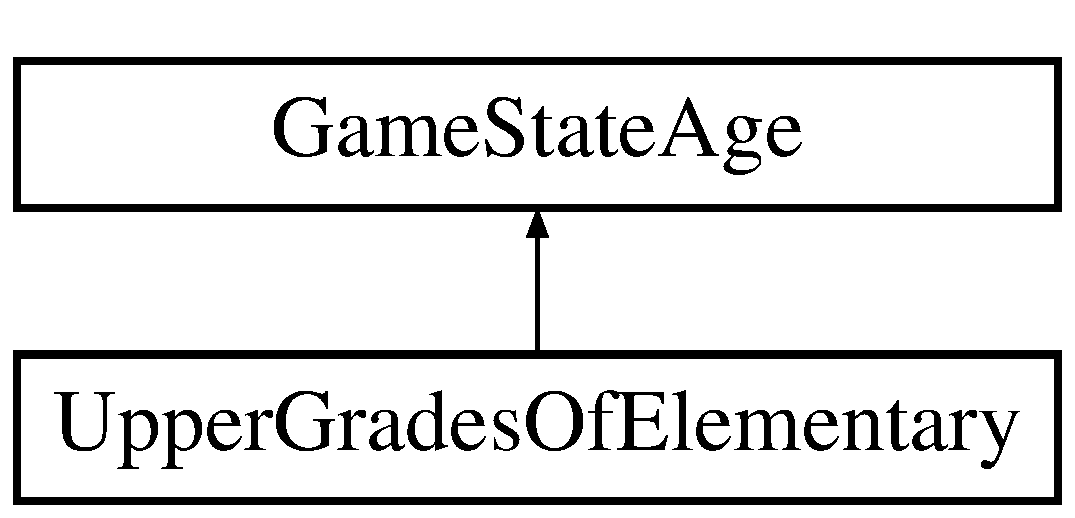
\includegraphics[height=2.000000cm]{class_upper_grades_of_elementary}
\end{center}
\end{figure}
\subsection*{Public メソッド}
\begin{DoxyCompactItemize}
\item 
\hyperlink{class_upper_grades_of_elementary_adc70033284a3d55dc45077eb7ecc789f}{Upper\-Grades\-Of\-Elementary} ()
\item 
void \hyperlink{class_upper_grades_of_elementary_a73f1b6ecad28525d60d995765bc504d3}{Set\-Up} ()
\item 
\hyperlink{class_game_state_age}{Game\-State\-Age} $\ast$ \hyperlink{class_upper_grades_of_elementary_af772cfb5983b01fdc8b4f5073c6c0e82}{Next\-Age} ()
\item 
std\-::vector$<$ \hyperlink{class_heroine}{Heroine} $>$ \hyperlink{class_upper_grades_of_elementary_a2aff40b541c73636baa75a94bec898ba}{Generate\-Enable\-Heroine} ()
\item 
std\-::vector$<$ \hyperlink{class_action}{Action} $>$ \hyperlink{class_upper_grades_of_elementary_a5ccf297eb998d128f6a01bc210620ed2}{Generate\-Enable\-Action} ()
\end{DoxyCompactItemize}


\subsection{コンストラクタとデストラクタ}
\hypertarget{class_upper_grades_of_elementary_adc70033284a3d55dc45077eb7ecc789f}{\index{Upper\-Grades\-Of\-Elementary@{Upper\-Grades\-Of\-Elementary}!Upper\-Grades\-Of\-Elementary@{Upper\-Grades\-Of\-Elementary}}
\index{Upper\-Grades\-Of\-Elementary@{Upper\-Grades\-Of\-Elementary}!UpperGradesOfElementary@{Upper\-Grades\-Of\-Elementary}}
\subsubsection[{Upper\-Grades\-Of\-Elementary}]{\setlength{\rightskip}{0pt plus 5cm}{\bf Upper\-Grades\-Of\-Elementary\-::\-Upper\-Grades\-Of\-Elementary} (
\begin{DoxyParamCaption}
{}
\end{DoxyParamCaption}
)}}\label{class_upper_grades_of_elementary_adc70033284a3d55dc45077eb7ecc789f}


\subsection{関数}
\hypertarget{class_upper_grades_of_elementary_a5ccf297eb998d128f6a01bc210620ed2}{\index{Upper\-Grades\-Of\-Elementary@{Upper\-Grades\-Of\-Elementary}!Generate\-Enable\-Action@{Generate\-Enable\-Action}}
\index{Generate\-Enable\-Action@{Generate\-Enable\-Action}!UpperGradesOfElementary@{Upper\-Grades\-Of\-Elementary}}
\subsubsection[{Generate\-Enable\-Action}]{\setlength{\rightskip}{0pt plus 5cm}vector$<$ {\bf Action} $>$ {\bf Upper\-Grades\-Of\-Elementary\-::\-Generate\-Enable\-Action} (
\begin{DoxyParamCaption}
{}
\end{DoxyParamCaption}
)\hspace{0.3cm}{\ttfamily  \mbox{[}virtual\mbox{]}}}}\label{class_upper_grades_of_elementary_a5ccf297eb998d128f6a01bc210620ed2}


\hyperlink{class_game_state_age_ac705cfe596fd49e2eec5d8f430f7f848}{Game\-State\-Age}を実装しています。

\hypertarget{class_upper_grades_of_elementary_a2aff40b541c73636baa75a94bec898ba}{\index{Upper\-Grades\-Of\-Elementary@{Upper\-Grades\-Of\-Elementary}!Generate\-Enable\-Heroine@{Generate\-Enable\-Heroine}}
\index{Generate\-Enable\-Heroine@{Generate\-Enable\-Heroine}!UpperGradesOfElementary@{Upper\-Grades\-Of\-Elementary}}
\subsubsection[{Generate\-Enable\-Heroine}]{\setlength{\rightskip}{0pt plus 5cm}vector$<$ {\bf Heroine} $>$ {\bf Upper\-Grades\-Of\-Elementary\-::\-Generate\-Enable\-Heroine} (
\begin{DoxyParamCaption}
{}
\end{DoxyParamCaption}
)\hspace{0.3cm}{\ttfamily  \mbox{[}virtual\mbox{]}}}}\label{class_upper_grades_of_elementary_a2aff40b541c73636baa75a94bec898ba}


\hyperlink{class_game_state_age_a0651ca176cb1e55c4f055aa3907e2165}{Game\-State\-Age}を実装しています。

\hypertarget{class_upper_grades_of_elementary_af772cfb5983b01fdc8b4f5073c6c0e82}{\index{Upper\-Grades\-Of\-Elementary@{Upper\-Grades\-Of\-Elementary}!Next\-Age@{Next\-Age}}
\index{Next\-Age@{Next\-Age}!UpperGradesOfElementary@{Upper\-Grades\-Of\-Elementary}}
\subsubsection[{Next\-Age}]{\setlength{\rightskip}{0pt plus 5cm}{\bf Game\-State\-Age} $\ast$ {\bf Upper\-Grades\-Of\-Elementary\-::\-Next\-Age} (
\begin{DoxyParamCaption}
{}
\end{DoxyParamCaption}
)\hspace{0.3cm}{\ttfamily  \mbox{[}virtual\mbox{]}}}}\label{class_upper_grades_of_elementary_af772cfb5983b01fdc8b4f5073c6c0e82}


\hyperlink{class_game_state_age_a21f816167d66266b8c234b40dff4a151}{Game\-State\-Age}を実装しています。

\hypertarget{class_upper_grades_of_elementary_a73f1b6ecad28525d60d995765bc504d3}{\index{Upper\-Grades\-Of\-Elementary@{Upper\-Grades\-Of\-Elementary}!Set\-Up@{Set\-Up}}
\index{Set\-Up@{Set\-Up}!UpperGradesOfElementary@{Upper\-Grades\-Of\-Elementary}}
\subsubsection[{Set\-Up}]{\setlength{\rightskip}{0pt plus 5cm}void {\bf Upper\-Grades\-Of\-Elementary\-::\-Set\-Up} (
\begin{DoxyParamCaption}
{}
\end{DoxyParamCaption}
)\hspace{0.3cm}{\ttfamily  \mbox{[}virtual\mbox{]}}}}\label{class_upper_grades_of_elementary_a73f1b6ecad28525d60d995765bc504d3}


\hyperlink{class_game_state_age_ae2de22cab7976aebb807f228f69309a1}{Game\-State\-Age}を実装しています。



このクラスの説明は次のファイルから生成されました\-:\begin{DoxyCompactItemize}
\item 
Home\-Coming/\hyperlink{_upper_grades_of_elementary_8h}{Upper\-Grades\-Of\-Elementary.\-h}\item 
Home\-Coming/\hyperlink{_upper_grades_of_elementary_8cpp}{Upper\-Grades\-Of\-Elementary.\-cpp}\end{DoxyCompactItemize}

\chapter{ファイル}
\hypertarget{_action_8cpp}{\section{Home\-Coming/\-Action.cpp}
\label{_action_8cpp}\index{Home\-Coming/\-Action.\-cpp@{Home\-Coming/\-Action.\-cpp}}
}
{\ttfamily \#include $<$iostream$>$}\\*
{\ttfamily \#include \char`\"{}Action.\-h\char`\"{}}\\*
{\ttfamily \#include $<$fstream$>$}\\*
{\ttfamily \#include $<$map$>$}\\*

\hypertarget{_action_8h}{\section{Home\-Coming/\-Action.h}
\label{_action_8h}\index{Home\-Coming/\-Action.\-h@{Home\-Coming/\-Action.\-h}}
}
{\ttfamily \#include \char`\"{}Utility.\-h\char`\"{}}\\*
{\ttfamily \#include $<$string$>$}\\*
{\ttfamily \#include $<$vector$>$}\\*
\subsection*{構成}
\begin{DoxyCompactItemize}
\item 
class \hyperlink{class_action}{Action}
\end{DoxyCompactItemize}

\hypertarget{_action_table_data_8h}{\section{Home\-Coming/\-Action\-Table\-Data.h}
\label{_action_table_data_8h}\index{Home\-Coming/\-Action\-Table\-Data.\-h@{Home\-Coming/\-Action\-Table\-Data.\-h}}
}
{\ttfamily \#import $<$Foundation/\-Foundation.\-h$>$}\\*
{\ttfamily \#import \char`\"{}Action.\-h\char`\"{}}\\*
\subsection*{構成}
\begin{DoxyCompactItemize}
\item 
class \hyperlink{interface_action_table_data}{Action\-Table\-Data}
\end{DoxyCompactItemize}

\hypertarget{_action_table_data_8mm}{\section{Home\-Coming/\-Action\-Table\-Data.mm}
\label{_action_table_data_8mm}\index{Home\-Coming/\-Action\-Table\-Data.\-mm@{Home\-Coming/\-Action\-Table\-Data.\-mm}}
}
{\ttfamily \#import \char`\"{}Action\-Table\-Data.\-h\char`\"{}}\\*
{\ttfamily \#import \char`\"{}Utility.\-h\char`\"{}}\\*

\hypertarget{_app_delegate_8h}{\section{Home\-Coming/\-App\-Delegate.h}
\label{_app_delegate_8h}\index{Home\-Coming/\-App\-Delegate.\-h@{Home\-Coming/\-App\-Delegate.\-h}}
}
{\ttfamily \#import $<$Cocoa/\-Cocoa.\-h$>$}\\*
{\ttfamily \#import \char`\"{}Game.\-h\char`\"{}}\\*
{\ttfamily \#import $<$cstdlib$>$}\\*
{\ttfamily \#import \char`\"{}Command\-Menu\-Controller.\-h\char`\"{}}\\*
{\ttfamily \#import \char`\"{}Story\-Window\-Controller.\-h\char`\"{}}\\*
\subsection*{構成}
\begin{DoxyCompactItemize}
\item 
class \hyperlink{interface_app_delegate}{App\-Delegate}
\end{DoxyCompactItemize}

\hypertarget{_app_delegate_8mm}{\section{Home\-Coming/\-App\-Delegate.mm}
\label{_app_delegate_8mm}\index{Home\-Coming/\-App\-Delegate.\-mm@{Home\-Coming/\-App\-Delegate.\-mm}}
}
{\ttfamily \#import \char`\"{}App\-Delegate.\-h\char`\"{}}\\*

\hypertarget{_command_menu_controller_8h}{\section{Home\-Coming/\-Command\-Menu\-Controller.h}
\label{_command_menu_controller_8h}\index{Home\-Coming/\-Command\-Menu\-Controller.\-h@{Home\-Coming/\-Command\-Menu\-Controller.\-h}}
}
{\ttfamily \#import $<$Cocoa/\-Cocoa.\-h$>$}\\*
{\ttfamily \#import \char`\"{}App\-Delegate.\-h\char`\"{}}\\*
{\ttfamily \#include \char`\"{}Action.\-h\char`\"{}}\\*
\subsection*{構成}
\begin{DoxyCompactItemize}
\item 
class \hyperlink{interface_command_menu_controller}{Command\-Menu\-Controller}
\end{DoxyCompactItemize}

\hypertarget{_command_menu_controller_8mm}{\section{Home\-Coming/\-Command\-Menu\-Controller.mm}
\label{_command_menu_controller_8mm}\index{Home\-Coming/\-Command\-Menu\-Controller.\-mm@{Home\-Coming/\-Command\-Menu\-Controller.\-mm}}
}
{\ttfamily \#import \char`\"{}Command\-Menu\-Controller.\-h\char`\"{}}\\*
{\ttfamily \#import \char`\"{}Action\-Table\-Data.\-h\char`\"{}}\\*
{\ttfamily \#import \char`\"{}Heroine\-Table\-Data.\-h\char`\"{}}\\*

\hypertarget{_game_8cpp}{\section{Home\-Coming/\-Game.cpp}
\label{_game_8cpp}\index{Home\-Coming/\-Game.\-cpp@{Home\-Coming/\-Game.\-cpp}}
}
{\ttfamily \#include $<$iostream$>$}\\*
{\ttfamily \#include \char`\"{}Game.\-h\char`\"{}}\\*
{\ttfamily \#include $<$cstdlib$>$}\\*
{\ttfamily \#include $<$vector$>$}\\*
{\ttfamily \#include \char`\"{}Utility.\-h\char`\"{}}\\*

\hypertarget{_game_8h}{\section{Home\-Coming/\-Game.h}
\label{_game_8h}\index{Home\-Coming/\-Game.\-h@{Home\-Coming/\-Game.\-h}}
}
{\ttfamily \#include \char`\"{}Hero.\-h\char`\"{}}\\*
{\ttfamily \#include \char`\"{}Heroine.\-h\char`\"{}}\\*
{\ttfamily \#include \char`\"{}Action.\-h\char`\"{}}\\*
{\ttfamily \#include \char`\"{}Lower\-Grades\-Of\-Elementary.\-h\char`\"{}}\\*
{\ttfamily \#include $<$vector$>$}\\*
{\ttfamily \#include $<$string$>$}\\*
\subsection*{構成}
\begin{DoxyCompactItemize}
\item 
class \hyperlink{class_game}{Game}
\end{DoxyCompactItemize}

\hypertarget{_game_state_age_8h}{\section{Home\-Coming/\-Game\-State\-Age.h}
\label{_game_state_age_8h}\index{Home\-Coming/\-Game\-State\-Age.\-h@{Home\-Coming/\-Game\-State\-Age.\-h}}
}
{\ttfamily \#include \char`\"{}Action.\-h\char`\"{}}\\*
{\ttfamily \#include \char`\"{}Heroine.\-h\char`\"{}}\\*
\subsection*{構成}
\begin{DoxyCompactItemize}
\item 
class \hyperlink{class_game_state_age}{Game\-State\-Age}
\end{DoxyCompactItemize}

\hypertarget{_hero_8h}{\section{Home\-Coming/\-Hero.h}
\label{_hero_8h}\index{Home\-Coming/\-Hero.\-h@{Home\-Coming/\-Hero.\-h}}
}
{\ttfamily \#include $<$string$>$}\\*
\subsection*{構成}
\begin{DoxyCompactItemize}
\item 
class \hyperlink{class_hero}{Hero}
\end{DoxyCompactItemize}

\hypertarget{_heroine_8h}{\section{Home\-Coming/\-Heroine.h}
\label{_heroine_8h}\index{Home\-Coming/\-Heroine.\-h@{Home\-Coming/\-Heroine.\-h}}
}
{\ttfamily \#include $<$string$>$}\\*
{\ttfamily \#include $<$vector$>$}\\*
\subsection*{構成}
\begin{DoxyCompactItemize}
\item 
class \hyperlink{class_heroine_attr}{Heroine\-Attr}
\item 
class \hyperlink{class_heroine}{Heroine}
\end{DoxyCompactItemize}

\hypertarget{_heroine_table_data_8h}{\section{Home\-Coming/\-Heroine\-Table\-Data.h}
\label{_heroine_table_data_8h}\index{Home\-Coming/\-Heroine\-Table\-Data.\-h@{Home\-Coming/\-Heroine\-Table\-Data.\-h}}
}
{\ttfamily \#import $<$Foundation/\-Foundation.\-h$>$}\\*
{\ttfamily \#include \char`\"{}Heroine.\-h\char`\"{}}\\*
\subsection*{構成}
\begin{DoxyCompactItemize}
\item 
class \hyperlink{interface_heroine_table_data}{Heroine\-Table\-Data}
\end{DoxyCompactItemize}

\hypertarget{_heroine_table_data_8m}{\section{Home\-Coming/\-Heroine\-Table\-Data.m}
\label{_heroine_table_data_8m}\index{Home\-Coming/\-Heroine\-Table\-Data.\-m@{Home\-Coming/\-Heroine\-Table\-Data.\-m}}
}
{\ttfamily \#import \char`\"{}Heroine\-Table\-Data.\-h\char`\"{}}\\*
{\ttfamily \#include \char`\"{}Utility.\-h\char`\"{}}\\*

\hypertarget{_lower_grades_of_elementary_8cpp}{\section{Home\-Coming/\-Lower\-Grades\-Of\-Elementary.cpp}
\label{_lower_grades_of_elementary_8cpp}\index{Home\-Coming/\-Lower\-Grades\-Of\-Elementary.\-cpp@{Home\-Coming/\-Lower\-Grades\-Of\-Elementary.\-cpp}}
}
{\ttfamily \#include $<$iostream$>$}\\*
{\ttfamily \#include \char`\"{}Lower\-Grades\-Of\-Elementary.\-h\char`\"{}}\\*

\hypertarget{_lower_grades_of_elementary_8h}{\section{Home\-Coming/\-Lower\-Grades\-Of\-Elementary.h}
\label{_lower_grades_of_elementary_8h}\index{Home\-Coming/\-Lower\-Grades\-Of\-Elementary.\-h@{Home\-Coming/\-Lower\-Grades\-Of\-Elementary.\-h}}
}
{\ttfamily \#include \char`\"{}Game\-State\-Age.\-h\char`\"{}}\\*
{\ttfamily \#include $<$vector$>$}\\*
{\ttfamily \#include \char`\"{}Heroine.\-h\char`\"{}}\\*
{\ttfamily \#include \char`\"{}Action.\-h\char`\"{}}\\*
\subsection*{構成}
\begin{DoxyCompactItemize}
\item 
class \hyperlink{class_lower_grades_of_elementary}{Lower\-Grades\-Of\-Elementary}
\end{DoxyCompactItemize}

\hypertarget{main_8mm}{\section{Home\-Coming/main.mm}
\label{main_8mm}\index{Home\-Coming/main.\-mm@{Home\-Coming/main.\-mm}}
}
{\ttfamily \#import $<$Cocoa/\-Cocoa.\-h$>$}\\*
\subsection*{関数}
\begin{DoxyCompactItemize}
\item 
int \hyperlink{main_8mm_a0ddf1224851353fc92bfbff6f499fa97}{main} (int argc, char $\ast$argv\mbox{[}$\,$\mbox{]})
\end{DoxyCompactItemize}


\subsection{関数}
\hypertarget{main_8mm_a0ddf1224851353fc92bfbff6f499fa97}{\index{main.\-mm@{main.\-mm}!main@{main}}
\index{main@{main}!main.mm@{main.\-mm}}
\subsubsection[{main}]{\setlength{\rightskip}{0pt plus 5cm}int {\bf main} (
\begin{DoxyParamCaption}
\item[{int}]{argc, }
\item[{char $\ast$}]{argv\mbox{[}$\,$\mbox{]}}
\end{DoxyParamCaption}
)}}\label{main_8mm_a0ddf1224851353fc92bfbff6f499fa97}

\hypertarget{_school_8h}{\section{Home\-Coming/\-School.h}
\label{_school_8h}\index{Home\-Coming/\-School.\-h@{Home\-Coming/\-School.\-h}}
}
{\ttfamily \#include $<$string$>$}\\*
\subsection*{構成}
\begin{DoxyCompactItemize}
\item 
class \hyperlink{class_school}{School}
\end{DoxyCompactItemize}

\hypertarget{_story_8hpp}{\section{Home\-Coming/\-Story.hpp}
\label{_story_8hpp}\index{Home\-Coming/\-Story.\-hpp@{Home\-Coming/\-Story.\-hpp}}
}
{\ttfamily \#include $<$vector$>$}\\*
{\ttfamily \#include $<$string$>$}\\*
\subsection*{構成}
\begin{DoxyCompactItemize}
\item 
class \hyperlink{class_story}{Story}
\end{DoxyCompactItemize}

\hypertarget{_story_view_8h}{\section{Home\-Coming/\-Story\-View.h}
\label{_story_view_8h}\index{Home\-Coming/\-Story\-View.\-h@{Home\-Coming/\-Story\-View.\-h}}
}
{\ttfamily \#import $<$Cocoa/\-Cocoa.\-h$>$}\\*
{\ttfamily \#import $<$vector$>$}\\*
{\ttfamily \#import $<$string$>$}\\*
\subsection*{構成}
\begin{DoxyCompactItemize}
\item 
class \hyperlink{interface_story_view}{Story\-View}
\end{DoxyCompactItemize}

\hypertarget{_story_view_8mm}{\section{Home\-Coming/\-Story\-View.mm}
\label{_story_view_8mm}\index{Home\-Coming/\-Story\-View.\-mm@{Home\-Coming/\-Story\-View.\-mm}}
}
{\ttfamily \#import \char`\"{}Story\-View.\-h\char`\"{}}\\*

\hypertarget{_story_window_controller_8h}{\section{Home\-Coming/\-Story\-Window\-Controller.h}
\label{_story_window_controller_8h}\index{Home\-Coming/\-Story\-Window\-Controller.\-h@{Home\-Coming/\-Story\-Window\-Controller.\-h}}
}
{\ttfamily \#import $<$Cocoa/\-Cocoa.\-h$>$}\\*
{\ttfamily \#import \char`\"{}Story\-View.\-h\char`\"{}}\\*
\subsection*{構成}
\begin{DoxyCompactItemize}
\item 
class \hyperlink{interface_story_window_controller}{Story\-Window\-Controller}
\end{DoxyCompactItemize}

\hypertarget{_story_window_controller_8mm}{\section{Home\-Coming/\-Story\-Window\-Controller.mm}
\label{_story_window_controller_8mm}\index{Home\-Coming/\-Story\-Window\-Controller.\-mm@{Home\-Coming/\-Story\-Window\-Controller.\-mm}}
}
{\ttfamily \#import \char`\"{}Story\-Window\-Controller.\-h\char`\"{}}\\*

\hypertarget{_system_8h}{\section{Home\-Coming/\-System.h}
\label{_system_8h}\index{Home\-Coming/\-System.\-h@{Home\-Coming/\-System.\-h}}
}
\subsection*{構成}
\begin{DoxyCompactItemize}
\item 
class \hyperlink{class_system}{System}
\end{DoxyCompactItemize}

\hypertarget{_upper_grades_of_elementary_8cpp}{\section{Home\-Coming/\-Upper\-Grades\-Of\-Elementary.cpp}
\label{_upper_grades_of_elementary_8cpp}\index{Home\-Coming/\-Upper\-Grades\-Of\-Elementary.\-cpp@{Home\-Coming/\-Upper\-Grades\-Of\-Elementary.\-cpp}}
}
{\ttfamily \#include $<$iostream$>$}\\*
{\ttfamily \#include \char`\"{}Upper\-Grades\-Of\-Elementary.\-h\char`\"{}}\\*

\hypertarget{_upper_grades_of_elementary_8h}{\section{Home\-Coming/\-Upper\-Grades\-Of\-Elementary.h}
\label{_upper_grades_of_elementary_8h}\index{Home\-Coming/\-Upper\-Grades\-Of\-Elementary.\-h@{Home\-Coming/\-Upper\-Grades\-Of\-Elementary.\-h}}
}
{\ttfamily \#include \char`\"{}Game\-State\-Age.\-h\char`\"{}}\\*
{\ttfamily \#include $<$vector$>$}\\*
{\ttfamily \#include \char`\"{}Heroine.\-h\char`\"{}}\\*
{\ttfamily \#include \char`\"{}Action.\-h\char`\"{}}\\*
\subsection*{構成}
\begin{DoxyCompactItemize}
\item 
class \hyperlink{class_upper_grades_of_elementary}{Upper\-Grades\-Of\-Elementary}
\end{DoxyCompactItemize}

\hypertarget{_utility_8h}{\section{Home\-Coming/\-Utility.h}
\label{_utility_8h}\index{Home\-Coming/\-Utility.\-h@{Home\-Coming/\-Utility.\-h}}
}
{\ttfamily \#include $<$string$>$}\\*
{\ttfamily \#include $<$fstream$>$}\\*
{\ttfamily \#include $<$vector$>$}\\*
{\ttfamily \#include $<$iostream$>$}\\*
\subsection*{構成}
\begin{DoxyCompactItemize}
\item 
struct \hyperlink{struct_range_number}{Range\-Number}
\end{DoxyCompactItemize}

\printindex
\end{document}
